
\chapter{Experiments and Discussion}

\section{Introduction}
In this chapter, we perform different experiments for the following purposes:
\begin{itemize}
	\item to evaluate the performance of uncertainty estimation of dropout variational inference and its variants as well as Laplace approximation. Comparisons and analysis towards the results of these two kinds of approach are given.
	
	\item to evaluate performance of training a domain specific classifier, with different strategies for collecting training data including manual labeling and automatic labeling, where the latter one is chosen based on uncertainty estimation.
	
	\item to evaluate performance of classifier including context information via CRF.
\end{itemize}

Before looking into the results, we need to specify the details of experiments such as the dataset, evaluation metrics. Besides, the detailed parameters of the model will be reported in section of each experiment to avoid confusions. Models were implemented in Tensorflow\cite{abadi2016tensorflow}, and optimization was performed using RMSprop with initial learning rate of $1e^{-5}$ and L2 regularization with coefficient of $3.5e^{-6}$ as well dropout regularization with coefficient of $1.0e^{-5}$. We used early stopping with all methods, where the amount of epochs to run was determined based on performance on a validation set. We set the number of maximum epoch as 20.

\newpage
\subsection{Dataset}
\paragraph{WRGBD\cite{lai2011large}} This dataset is a public large-scale dataset of 300 household objects captured from multi-viewpoint. The objects are organized into 51 categories and 300 instance classes in hierarchical structure. There are multiple instances in different categories. Each object was placed on a turn table and captured from a systematically sampled view hemisphere with $15^{\circ}$ step in elevation (from $30^{\circ}$to $60^{\circ}$) and $2^\circ$ step in azimuth (from $0^\circ$ to $360^\circ$) (cf. figure \ref{fig:wrgbd2}). The total size of entire dataset is around $160.9\times10^3$. To note that category level recognition involves classifying objects with similar semantic appearance such as cereal boxes with different texture into same category, instead of just physical appearance. Instance level recognition is to classify objects with similar physical appearance to the same category. Therefore the overlapping in features space between classes in category recognition is larger than that in instance recognition. More abstract and semantic concepts are expected to be learned in category recognition.  

\paragraph{UniHB} To simulate application-specific situation in deployment of robots, we recorded a similar dataset by putting objects on a turn table in front of the robot and recording partial views of objects. We follow the same methodology as \cite{lai2011large} suggests for WRGBD, but with only one object instance for each category in the dataset. This analogue of WRGBD dataset is called the IAI-ODU dataset of UniHB. In this work, we call it UniHB dataset for simplicity. The size of data with elevation $45^\circ$ is around $8.6\times10^3$ and that of data with elevation $30^\circ$ and $60^\circ$ is around $17.1\times10^3$.

While the UniHB dataset's setup strives to mimic the WRGBD one, the differing capturing conditions such as different equipment and light conditions even appearances of objects, result in obvious changes in feature space, thus yielding a significant drop on classification accuracy. In addition to the existing 51 categories, there are 28 novel objects(cf. figure \ref{fig:not_in_wrgbd}) that do not belong to the 51 class categories and these objects are treated as out-of-distribution(OOD) data for testing uncertainty estimation of the model. To note that data of these novel classes are recorded in a slight different way, that is, their view points are sampled with $15^{\circ}$ step in elevation (from $30^{\circ}$to $60^{\circ}$) and $5^\circ$ step in azimuth (from $0^\circ$ to $360^\circ$). The size of this OOD dataset is around $6.0\times10^3$.

% and are captured from a systematically sampled view sphere with $10^{\circ}$ step in elevation (from $85^\circ$ to $-85^\circ$) and $5^\circ$ step in azimuth

%Each test scene is captured from a systematically sampled view hemisphere with $10^{\circ}$ step in elevation (from $75^{\circ}$ to $15^{\circ}$) and $5^{\circ}$ step in azimuth.

\paragraph{T-LESS\cite{hodan2017tless}} This dataset features 30 commodity electrical parts which have no significant texture, discriminative color or distinctive reflectance properties, and often bear similarities in shape and/or size. Furthermore, a unique characteristic of the objects is that some of them are parts of others. All images were captured systematically sampled from a view sphere, resulting in around $38.0\times10^3$ training images and $10.0\times10^3$ test scene images (cf. figure \ref{fig:tless_test}). The training images depict objects in isolation with a black background, while the test images are from 20 table-top scenes with arbitrarily arranged objects placed on table. In this work we only consider the cropped images of objects in testing scenes, resulting a testing set with size $69.5\times10^3$. Nevertheless, the context information in the scene can be exploited with conditional random field in the next experiment.

Because objects in test scenes are mostly occluded and have different backgrounds and lightness. Therefore we employ data augmentation to improve the performance, where the real single objects are augmented and put onto different background images from VOC2012 dataset\cite{pascal-voc-2012}(cf. figure \ref{fig:tless_train}). Since collecting real data requires much manual effort, we want to first train classifier on synthetic data which are multi-view images of objects rendered from 3D reconstructed CAD models with similar augmentations as the real single objects(cf. figure \ref{fig:tless_train}). Although the real object and synthetic object do not look much different, there is significantly large domain gap between them such as texture and details on the object so that the performance of classifier trained on synthetic dataset on test set decreases a lot. One way to tackle this is that we can collect labeled data automatically based on improved uncertainty estimation, which can then be used to train a more accurate classifier.


 \begin{figure}[H]
 	\begin{center}
 		\includegraphics[height=10cm, width=16cm]{domain_diff}
 		\caption{Example of masked images of objects from 51 categories in WRGBD and UniHB dataset. In each category, the left is from WRGBD and the right is from UniHB. We randomly pick one instance for the objects of WRGBD. We can see some light and appearance difference between objects in these two datasets.}		
 		\label{fig:wrgbd2}
 	\end{center}
 \end{figure}

\begin{figure}[H]
	\begin{center}
		\includegraphics[height=7cm, width=12cm]{not_in_wrgbd}
		\caption{Example of masked images of objects from 28 categories which are not belonging to WRGBD categories, which are treated as OOD data samples.}		
		\label{fig:not_in_wrgbd}
	\end{center}
\end{figure} 

\begin{figure}[H]
	\begin{center}
		\includegraphics[height=8.5cm, width=14cm]{tless_trn_test}
		\caption{Example of object of each category in original training set and test set. In each thumbnail, the left image is real single object with black background and the right image is cropped image of object in test scene.}		
		\label{fig:tless_test}
	\end{center}
\end{figure} 

\begin{figure}[H]
		\centering
		\includegraphics[height=9cm, width=16cm]{tless_domain_diff}
		\caption{Example of object of each category with augmentation. In each thumbnail, the left image is real augmented object and the right image is synthetic augmented object.}		
		\label{fig:tless_train}
\end{figure} 


\subsection{Uncertainty measures}
For each prediction, we can obtain one predictive probability distribution from our model with equation \ref{marginalization_test}. In order to quantify uncertainty of the prediction, there are different metrics to measure the uncertainty of prediction, which are introduced in the following. We define $x^\star$ as one test data sample and $\mathcal D$ as our training set. 
\paragraph{Confidence} is defined as the maximum probability of the output predictive distribution, whose index is the class prediction.

\begin{equation}\label{confidence}	
\begin{aligned}
conf = \max_c \big[ p(y=c|x^\star, \mathcal D) \big]
\end{aligned}
\end{equation}
where $conf \in [0,1]$, $c \in \mathcal L = \{0,...,|\mathcal L|-1\}$, and $\mathcal L$ represents output space in which label is expressed as number index which is transformed into one-hot representation in computation of objective function. The larger this quantity is, the less uncertain the prediction is. 

\paragraph{Predictive entropy} is quantity that captures the average amount information contained in predictive distribution\cite{shannon1948mathematical}: 
\begin{equation}\label{entropy}	
\begin{aligned}
\mathcal H[p(y|x^\star, \mathcal D)] = -\sum_{c}p(y=c|x^\star, \mathcal D)\text{log}p(y=c|x^\star, \mathcal D)
\end{aligned}
\end{equation}
where $c$ is the possible class $y$ can take, $\mathcal H(\cdot) \in [0, \text{log}{|\mathcal P|}]$, the larger this quantity is, the more uncertain the prediction is.

\paragraph{Mutual information}
Mutual information between the prediction $y$ and the weights posterior offers a different uncertainty measure when compared with the aforementioned ones. This measure is widely used in active learning tasks\cite{houlsby2011bayesian}, which is also called Bayesian active learning disagreement(BALD). The definition of this measure is as follows:
\begin{equation}\label{mi}	
\begin{aligned}
\mathcal I[y,\bld \omega|x^\star, \mathcal D] &= \mathcal H[y|x^\star, \mathcal D] - \mathbb E_{p(\bld \omega| \mathcal D)}\big[\mathcal H[y|x^\star, \bld \omega] \big] \\
&= -\sum_{c}p(y=c|x^\star, \mathcal D)\text{log}p(y=c|x^\star, \mathcal D) \\ &+ \mathbb E_{p(\bld \omega|\mathcal D)}[-\sum_{c}p(y=c|x^\star, \bld \omega)\text{log}p(y=c|x^\star, \bld \omega)] \\
&\approx -\sum_{c}p(y=c|x^\star, \mathcal D)\text{log}p(y=c|x^\star, \mathcal D) \\ &+ \mathbb E_{q(\bld \omega)}[-\sum_{c}p(y=c|x^\star, \bld \omega)\text{log}p(y=c|x^\star, \bld \omega)]
\end{aligned}
\end{equation}
where $\mathcal I(\cdot) \in [0,\text{log}{|\mathcal P|}]$.
This quantity considers the effect of approximate posterior distribution more directly. Compared with aforementioned uncertainty measures, this one should be able to capture the model uncertainty more accurately. To think about it intuitively, this quantity measures the information gain between the entropy of predictive output distribution and the expected entropy of output distribution wr.t. weights posterior. It will be low only if the predictive distribution agrees with most of possible models(weights realizations), which means that the model is sure about its prediction. Otherwise, it will be high because most of possible models do not agree with the other models and thus the predictive distribution will be more uniform and thus has higher entropy.

\subsection{Evaluation metrics}
As is stated in \cite{gneiting2007probabilistic}, the goal of probabilistic prediction is to maximize the sharpness of predictive distribution subject to calibration. Calibration refers to the statistical consistency between the predictive probability and the occurrence of observations, which is the frequency of the event. Therefore we employ different metrics including both the accuracy and other quantities related to calibration as well as summary of accuracy and calibration. Additionally, we also employ histogram and diagram to express the results visually. While the visual one can show us the results more intuitively, the quantitative one can allow us to evaluate the results more objectively. The comparison between them may help us to examine if visual metrics are corresponding to the numerical metrics, which may provide more insights in evaluating uncertainty estimation. 

\paragraph{Uncertainty histogram} is a intuitive visual tool for analyzing the statistics of the uncertainty estimation. Compared with normal histogram, there is one difference to stress on. In order to make visual effect more clear and hence the analysis easier, \textbf{normalizer} of each type of prediction is the size of this type of predictions instead of size of all predictions. In detail, we have three types of prediction for plotting the histogram, which are:
 \begin{itemize}
 	\item \textbf{correct prediction}
 	\item \textbf{miss-classification}
 	\item \textbf{out-of-distribution(OOD)}
 \end{itemize}The range of y axis is $[0,1]$ because we normalize the number in each bin, and range of x axis is set by the range of corresponding type of uncertainty measure.

\paragraph{Reliability diagram(Calibration curve)} is another visual tool for expressing \textbf{calibration} performance of the model\cite{guo2017calibration}, which plots the frequency of success(accuracy of predictions in specific bin) as a function of confidence, which is predictive likelihood of prediction. If the model is perfectly calibrated, this function should be overlapping with the diagonal line exactly. The closer this curve is to diagonal curve, the better the calibration performance is. In order to draw the curve, we firstly group the predictions into $M$ interval bins w.r.t. confidence and then calculate the accuracy of predictions in each bin. We use $M=20$ in this work. To quantify the proximity to the diagonal curve, we use two metrics:
\begin{itemize}
	\item \textbf{Expectation calibration error(ECE)}: in order to obtain a more objective measure of calibration quality, we can compute the \textbf{expected calibration error} by computing the weighted average of difference between accuracy and confidence:
	
	\begin{equation}
	ECE = \sum_{m=1}^{M}\frac{|B_m|}{n}|acc(B_m) - conf(B_m)|
	\end{equation}
	where $n$ is the number of samples, and $acc(B_m)$ represents the accuracy of samples, $conf(B_m)$ the average predicted confidence of samples in $m$-th bin. We can see that this metric measures the inconsistency between the statistics and predictive distribution. To note that this metric only considers the calibration quality instead of accuracy. One drawback of this metric is that, because the weights are computed based on number of samples in each bin, the metric would bias if most of predictions are clustering in few bins. Then the weights of these bins are much larger than other bins and other bins with large error would be ignored. 
	
	\item \textbf{Maximal calibration error(MCE)}:
	Considering the drawback mentioned in ECE, we make use of this metric. Additionally, in high risk applications where reliable confidence measures are absolutely necessary, we may wish to take the worst case into account. It is defined as follows:
	
	\begin{equation}
	MCE = \max_m|acc(B_m) - conf(B_m)|
	\end{equation}
\end{itemize}


\paragraph{Proper scoring rules:} 
Scoring rules provides a \textbf{summary} measure in the evaluation of probabilistic forecasts. It assigns a numerical score based on the difference between predictive distribution and real distribution. 

Because we want to make predictions for the future and also have a suitable measure of the uncertainty associated with them (see \cite{gneiting2007strictly} for a review). We can define the scoring rule as a function $\mathcal S(p(y|\bld x), (y|\bld x))$ that evaluates the quality of predictive distribution $p(y|\bld x)$ relative to an event $y|\bld x \sim q(y|\bld x)$ where $q(y|\bld x)$ represents the true distribution over $(y|\bld x)$. Consequently, the expected scoring rule is:

\begin{equation}\label{scoring rule}
	\mathcal S(p, q) = \int q(y| \bld x) \mathcal S(p,(y|\bld x))dy
\end{equation}

$\mathcal S(p,q)$ is proper if $\mathcal S(p,q) \leq S(q,q)$, with equality holds if and only if $p(y|\bld x) = q(y|\bld x)$. Here we adopt two simple and famous proper scoring rules in which the less it is, the better the performance is:
\begin{itemize}
	\item \textbf{averaged negative log likelihood(NLL)}:NLL is a popular metric for evaluating predictive uncertainty	\cite{quinonero2005evaluating}. This metric considers aforementioned confidence as likelihood. The smaller this metric is, the better the predictive distribution is.
	
	\begin{equation} \label{nll}
		NLL = -\frac{1}{|\mathcal D_{test}|}\sum_{i=1}^{|\mathcal D_{test}|}\text{log}(p(y_i = c_i|\bld x_i))
	\end{equation}
	where $c_i$ is the ground truth label for $\bld x_i$.	
	\item \textbf{Brier score} is the mean squared error between the target distribution(one-hot encoding label) and predictive distribution:
	
	\begin{equation} \label{bs}
	BS = -\frac{1}{|\mathcal D_{test}|}\sum_{i=1}^{|\mathcal D_{test}|}(\bld y^{gt}_i - p(\bld y_i|\bld x_i))^2
	\end{equation}
	where $\bld y^{gt}_i$ is the one-hot encoding ground truth label for $\bld x_i$. 
	
\end{itemize}

\paragraph{Separability metrics:} In addition to the summary metrics of predictive probability. We are also interested in the separability between different types of predictions, which can assist the down-stream tasks if they are highly separable (e.g. separate correct predictions and false predictions or out-of-distribution data to improve robustness of system and provide more safety guarantee). To note that, we treat the correct predictions as positive samples in the two following metrics.
\begin{itemize}
	\item \textbf{Area under Receiver Operating Characteristic curve(AUROC)}:Since one of our goals is to choose automatically labeled data based on uncertainty estimation, it's necessary to evaluate the separability between correct predictions and false predictions or out-of distribution data predictions. ROC curve describes the relationship between true positive rate($tpr=\frac{tp}{tp+fn}$) and false positive rate($fpr=\frac{fp}{fp+tn}$). Moreover, AUROC can be interpreted as the probability that a positive samples has a greater score than a negative samples. However, the drawback of AUROC is that, the normalizers of two kinds of rate in ROC curve are independent to each other. When these two normalizers differs too much. AUROC can provide misleading conclusion. For example, if the number of negative predictions is much higher than positive one, the AUROC could still achieve a relatively high value, while in fact there are already many false positives. 
	
	\item \textbf{Area under Precision Recall curve(AUPR)}: Considering the downside of AUROC, another evaluation metric is employed, that is AUPR. AUPR describes the relationship between precision($pr = \frac{tp}{tp+fp}$) and recall($tpr=\frac{tp}{tp+fn}$), which resolves the problem of different base number. In the previously mentioned case, though the AUROC is high, the AUPR will be low because the precision is low. 
\end{itemize}


\section{Uncertainty estimation experiments}

\subsection{Experiments \RNum{1}}
In this experiments, we want to evaluate our model on a relatively easy task which is instance recognition at first. That means, the appearances of different classes as well as the out-of-distribution data are highly discriminable. To this end, we separate WRGBD dataset into two subsets based on the instance class. Subset \RNum{1} contains objects with instance class from 0 to 199 (assuming that here we use index to denote the instance label) and Subset \RNum{2} contains objects with instance class from 200 to 299. 

We train our model with objects captured in elevation $30^\circ$ and $60^\circ$ of Subset \RNum{1} (in which we split off 20\% of training set as validation set for model selection in training). The size of training set and validation set is around $71.0\times10^3$. Then we test the model on objects captured in elevation $45^\circ$ of both Subset \RNum{1} and Subset \RNum{2}. In this experiment, the objects in Subset \RNum{2} serve as out-of-distribution samples because they are not present during training. The size of test set is around $35.6\times10^3$ and that of OOD dataset is around $17.8\times10^3$. 

In this experiment, we just want to test and compare the performance of different approaches. Because the OOD data is highly different to the training set. The model should express high uncertainty when facing these data. Nevertheless, the miss-classifications should have higher uncertainty than the correct predictions because the model should be confident when it makes predictions correctly. Otherwise the model is overconfident when it's confident with its incorrect predictions, which can induce hazardous consequence in some safety-critical applications. As we can see in the figure \ref{exp1_histo}, the original ResNet50 model is highly overconfident, which assigns high confidence to nearly $50\%$ of miss-classification and nearly $30\%$ of OOD data in the highest bin. While the model with concrete dropout and multi-drop can significantly decrease these two proportions. As we can see, different uncertainty show similar trend in this experiment.

In addition to uncertainty histogram, we also plot the calibration curve of each model evaluated on both test set and OOD dataset in figure \ref{exp1_reliability}. As expected, the calibration performance of original model is much worse than those of the other two models. This result is corresponding to the results in \cite{guo2017calibration}, that the model is highly overconfident. And the concrete dropout and multi-dropout can mitigate the undesired problem significantly.

\begin{figure}[H]
	\begin{center}
		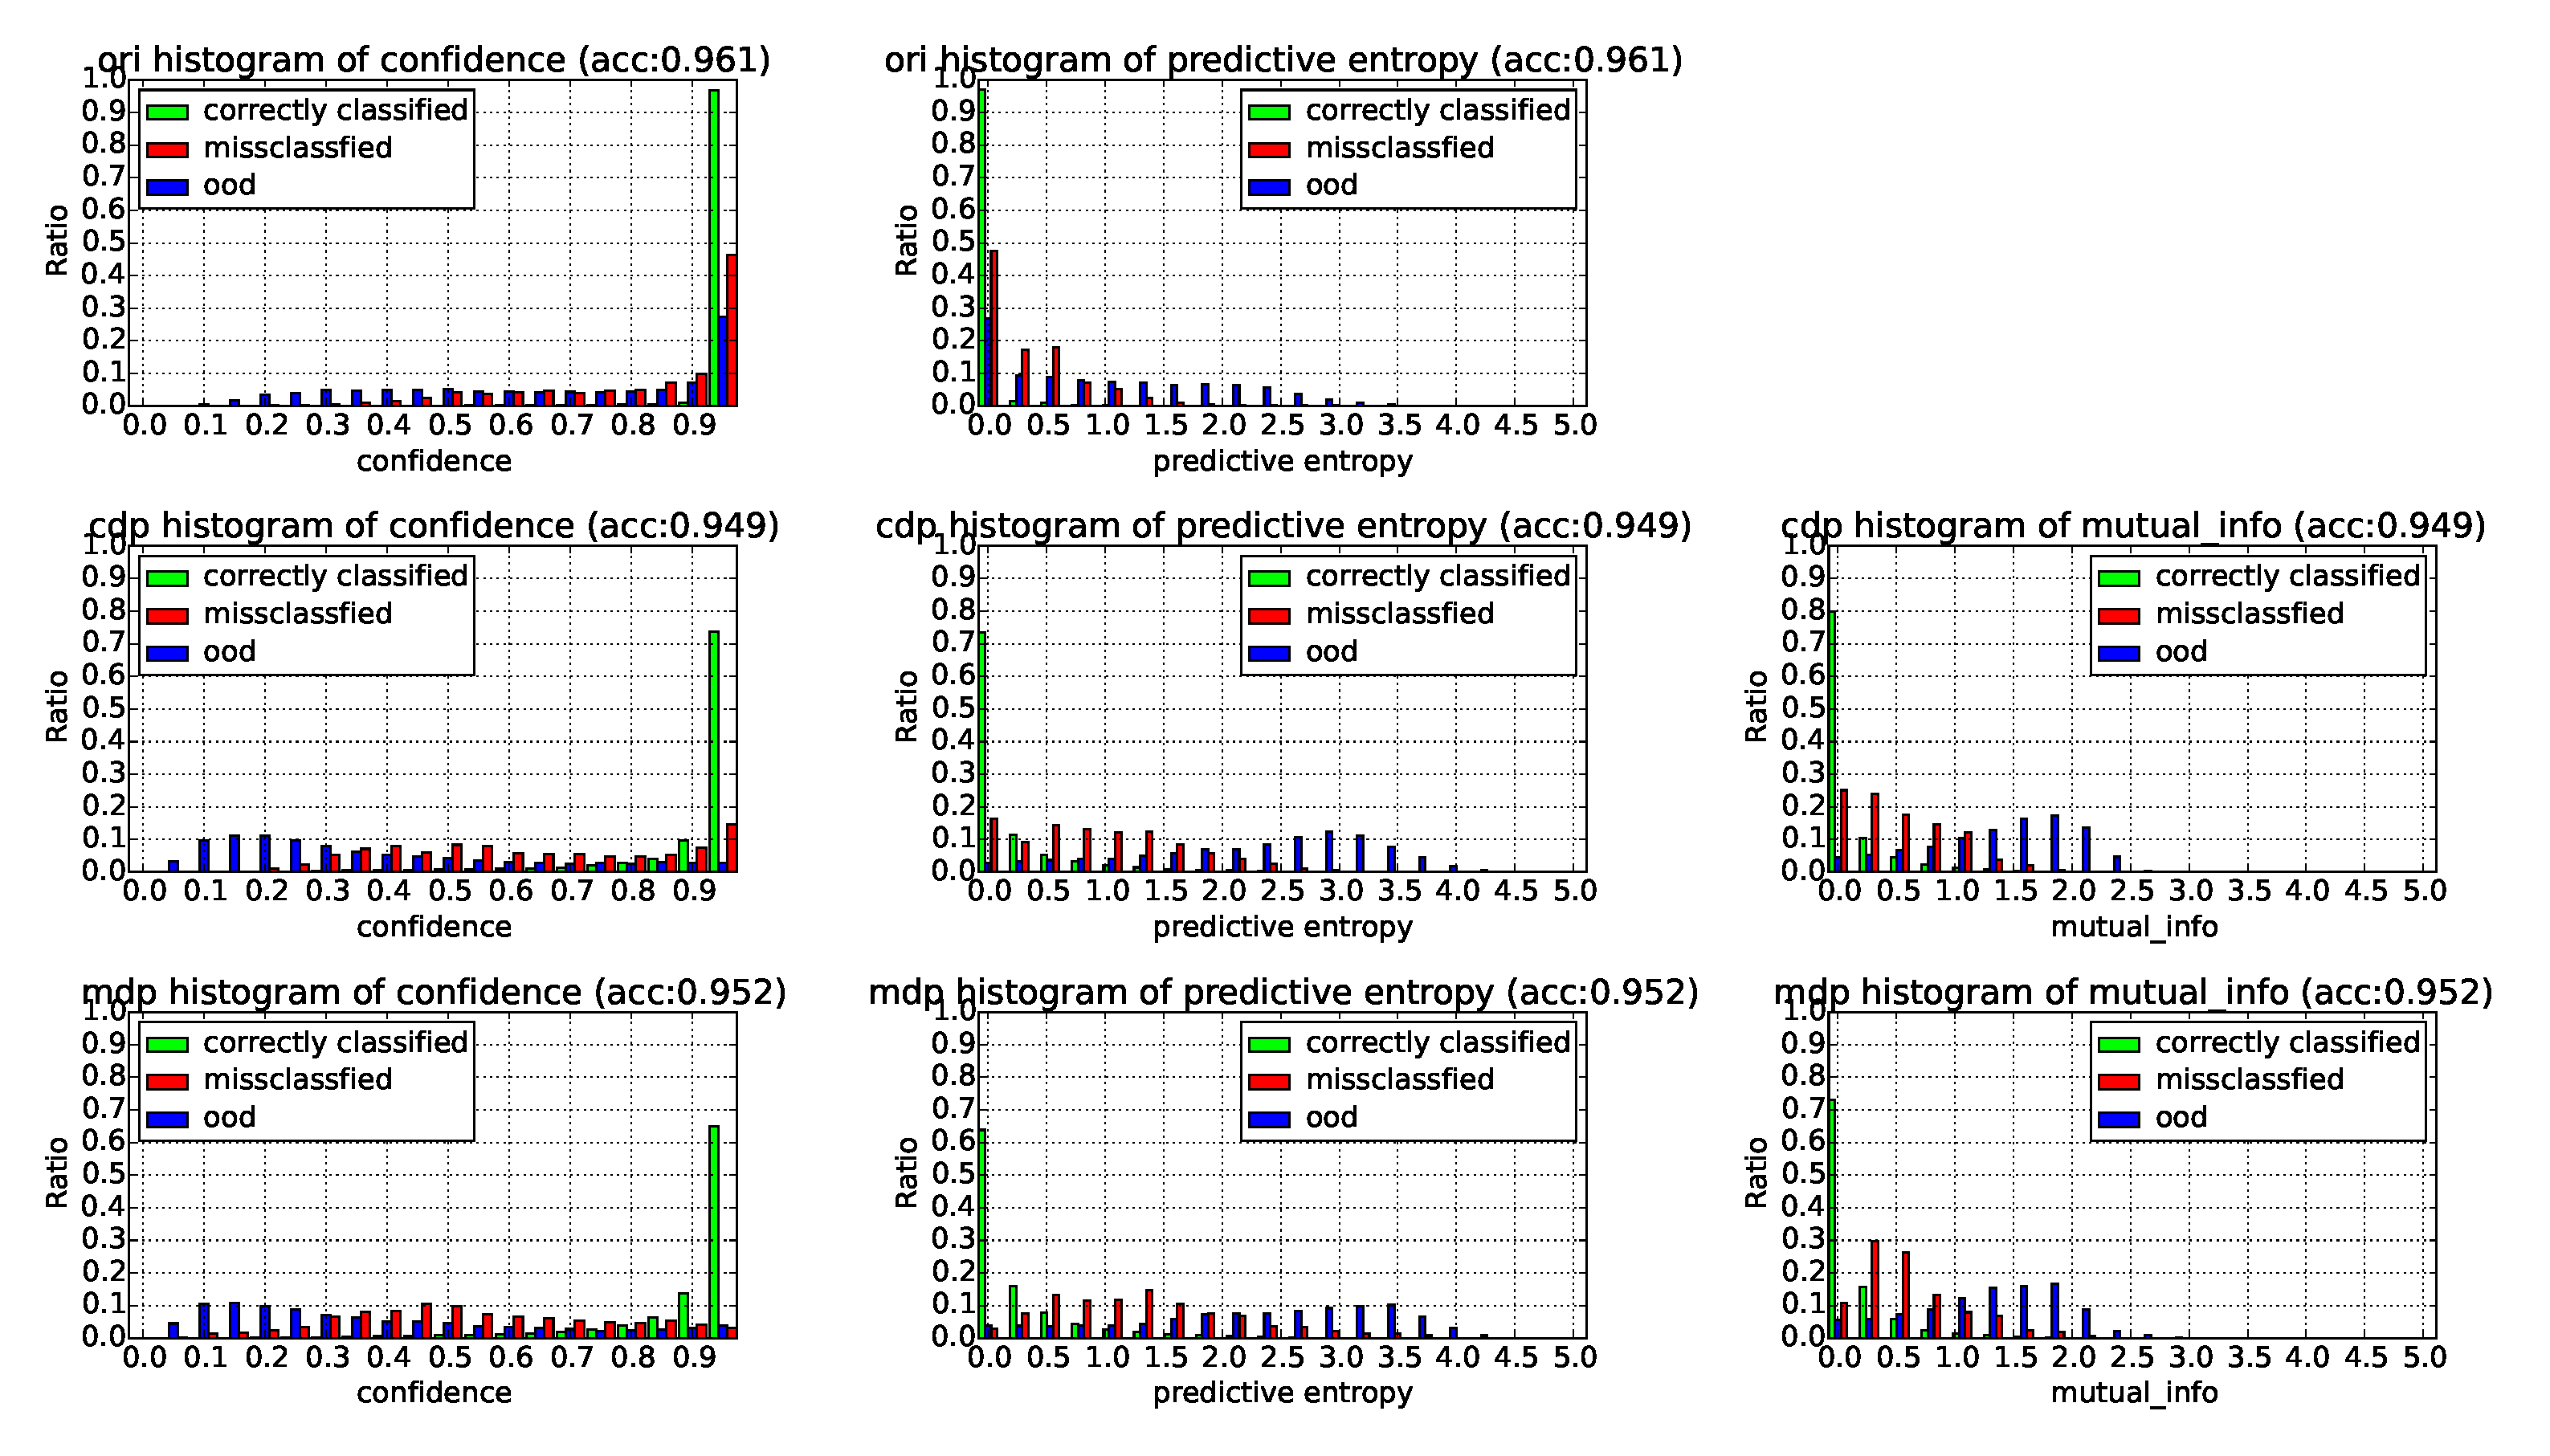
\includegraphics[height=7cm, width=16cm]{uncertainty_estimation/exp1/exp1_histo}
		\caption{Uncertainty(confidence, predictive entropy, mutual information) histograms of original ResNet50, ResNet50 with concrete dropout and ResNet50 with multi-dropout.}		
		\label{exp1_histo}
	\end{center}
\end{figure}
\begin{figure}[H]
	\begin{center}
		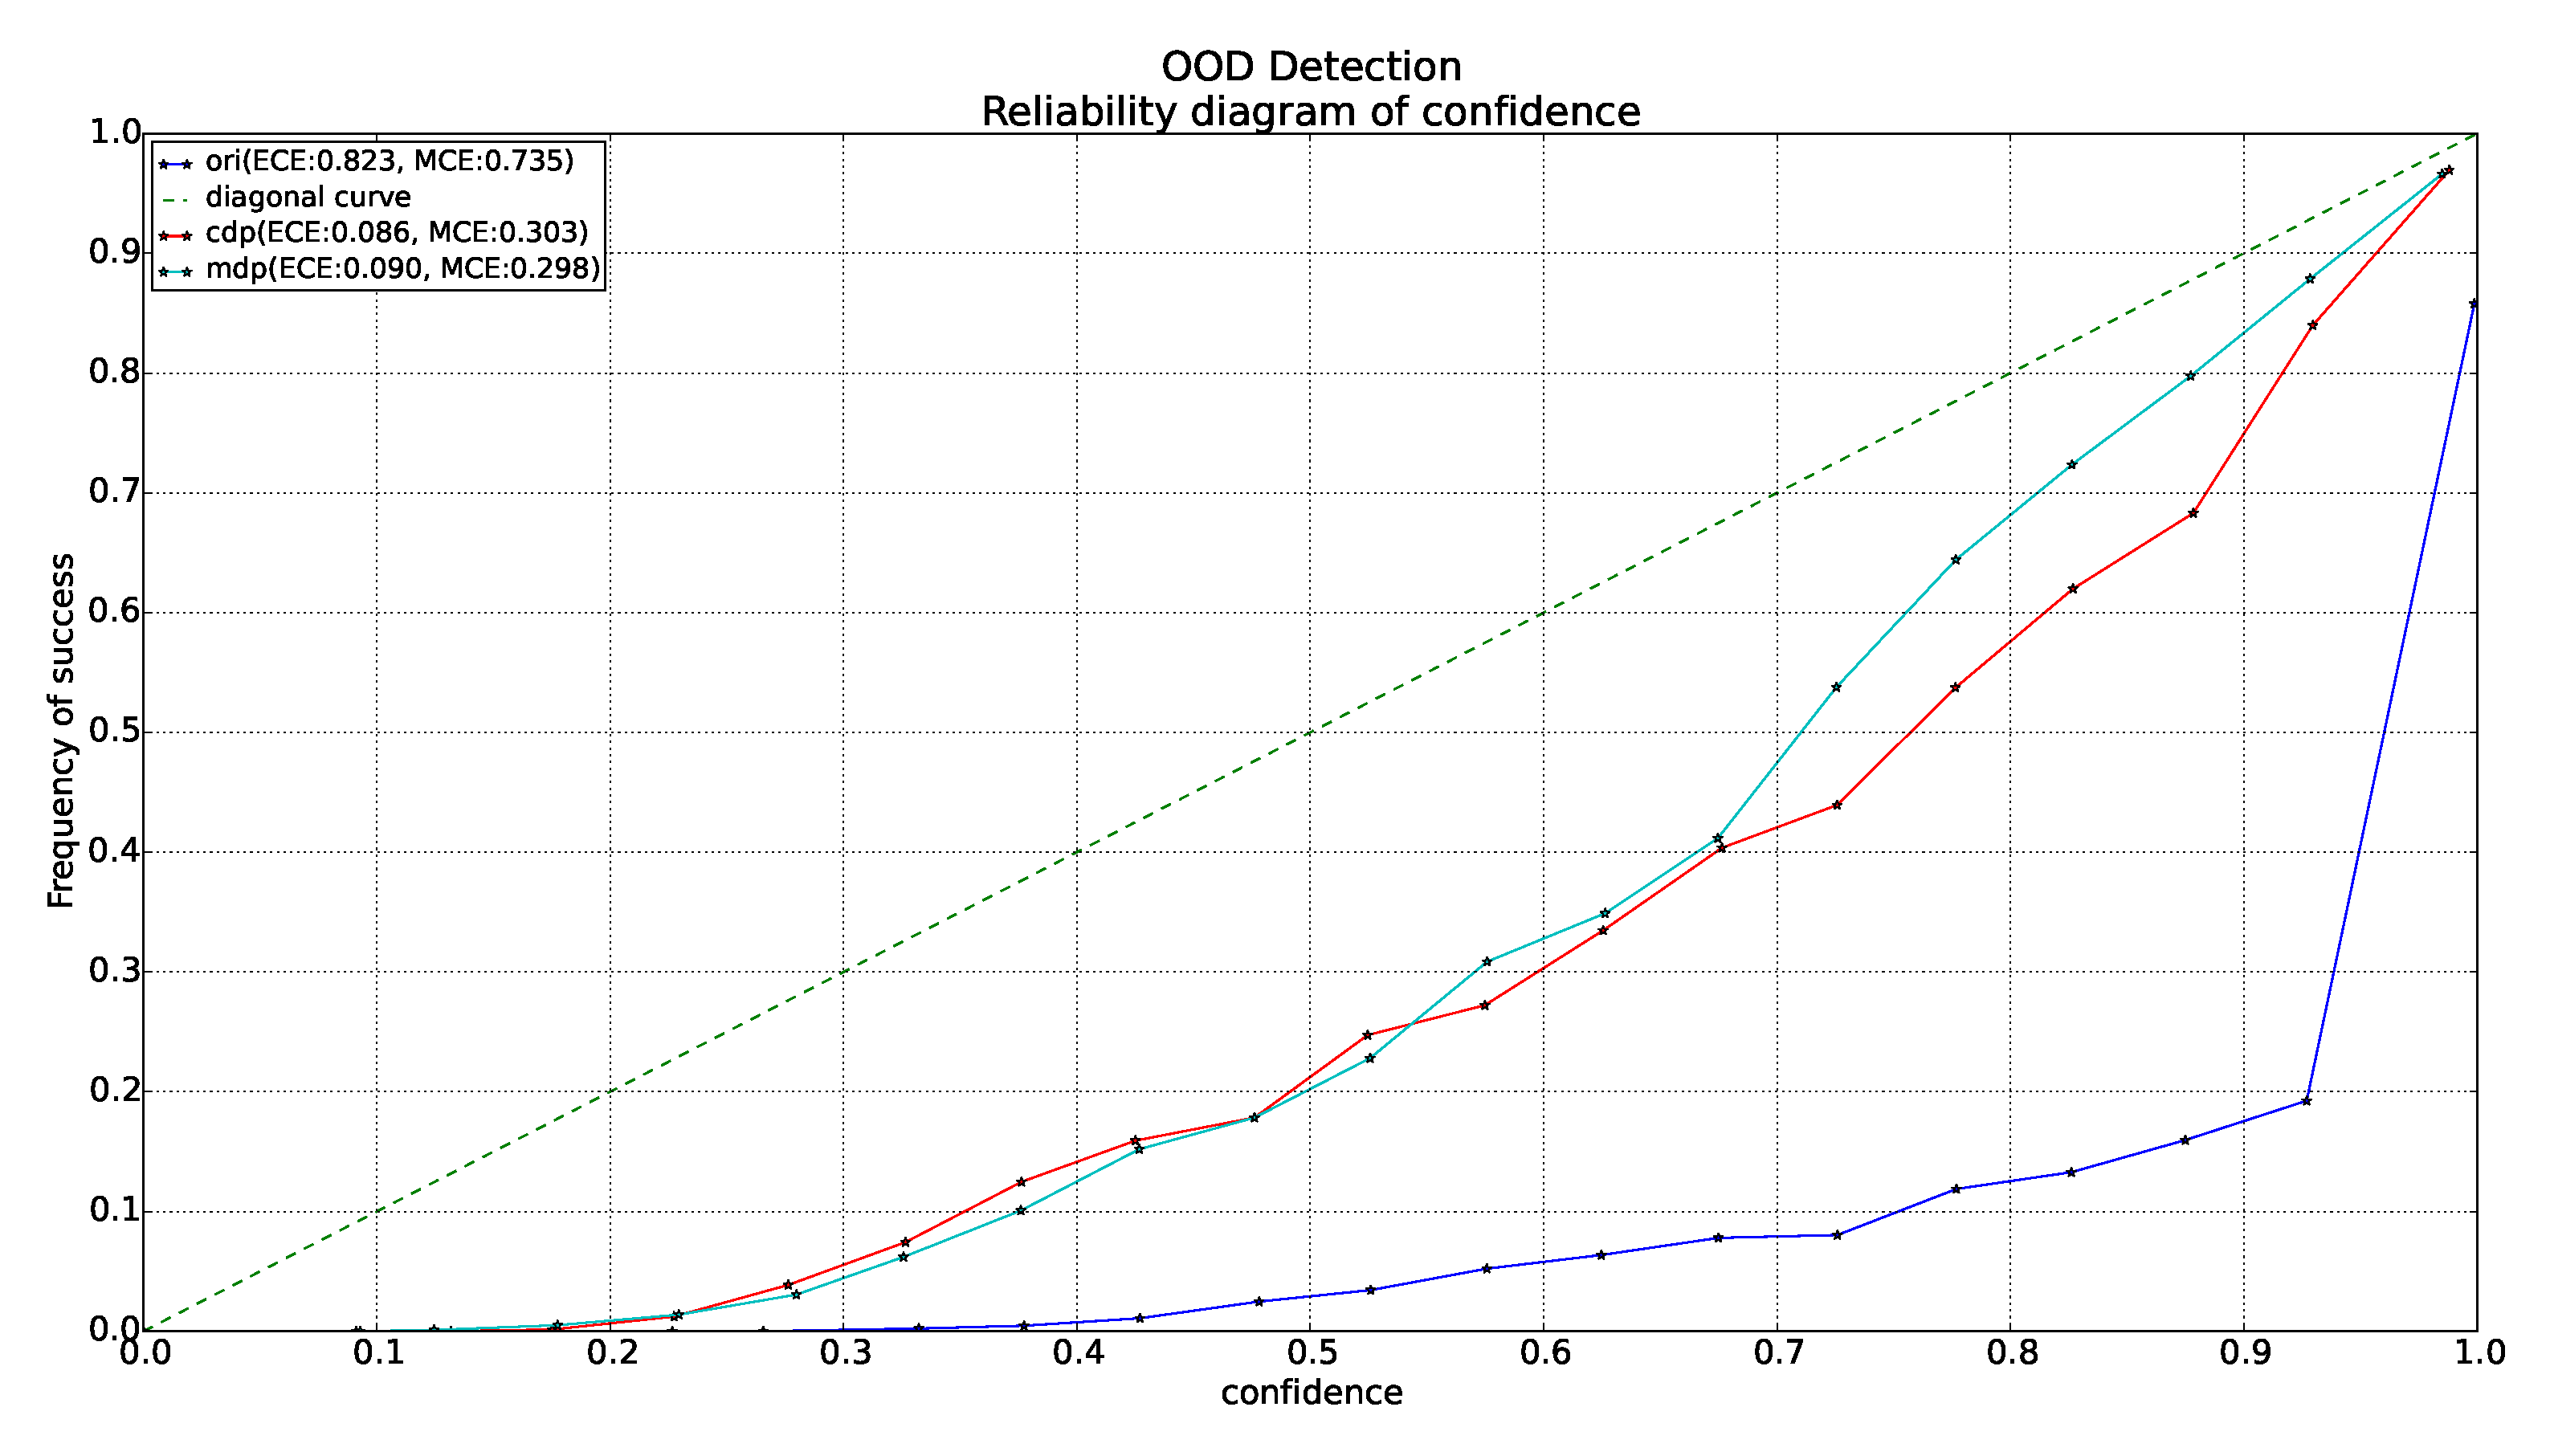
\includegraphics[height=6cm, width=12cm]{uncertainty_estimation/exp1/exp1_reliability}
		\caption{Calibration curves of original ResNet50, ResNet50 with concrete dropout and ResNet50 with multi-dropout.}		
		\label{exp1_reliability}
	\end{center}
\end{figure}

\newpage
\subsection{Experiments \RNum{2}}
In this experiment, we evaluate our model on a category recognition task. The difficulties are expressed in two-fold. Firstly, in this task, the model is confronted with classes with more overlapping. Second, because we want to simulate situation of deploying robots in real world scenario and facing data in real world, the UniHB dataset with domain gap(cf. figure\ref{fig:wrgbd2}) to WRGBD is used to achieve this goal. This means, the uncertainty estimation should not only be able to perform well on dataset with exactly same distribution to training set, but also to generalize well to dataset with domain gap which may decrease the accuracy significantly.

Accordingly, we use the entire WRGBD dataset including all view points, whose size is around $160.9\times10^3$, to train our model (in which we split off 20\% of training set as validation set for model selection during training). When it comes to UniHB dataset, we treat objects captured in elevation $30^\circ$ and $60^\circ$ in this dataset as \textbf{adaptation set}, whose size is around $17.1\times10^3$. We test performance of uncertainty estimation on this adaptation dataset. The images of $45^\circ$, whose size is around $8.6\times10^3$ , are used for final evaluation after we fine-tune the model with subset of adaptation set to obtain a domain specific model. The latter part will be experimented in next section. Besides, we also evaluate the uncertainty estimation on OOD dataset(cf. figure \ref{fig:not_in_wrgbd}) whose size is around $6.0\times10^3$. 

We firstly explain protocols in the following for different kinds of metric, which can help understanding the plots and extracting useful information more easily and quickly.  
\begin{itemize}
	\item The following visual metrics are chosen in one of three runs of different random seeds. The average quantitative results are given in tables following the visual metrics.
	\item The calibration curve with title "Classification" on the left is plotted \textbf{only} on predictions of test set. The one with title "OOD detection" on the right is plotted on predictions of \textbf{both} OOD dataset and test dataset.
	\item The ROC curve and PR curve measure the separability between two types of prediction.
	The ones with title "classification" on the left measure the separability between \textbf{correct prediction} and \textbf{miss-classification}. The ones with title "OOD detection" on the right measure the separability between \textbf{correct prediction} and \textbf{OOD prediction}. In all ROC curve and PR curve, correct prediction is always chosen to be positive.
	\item As is shown in uncertainty histogram, we have used three uncertainty measures. Each one has its own ROC curve and PR curve of correct prediction versus miss-classification or OOD prediction. In the following plots of ROC curve and PR curve, we only show the one with highest area under curve. In detail, \textbf{Confidence} is chosen in case of correct prediction versus miss-classification. \textbf{Mutual information} is chosen in case of correct prediction versus OOD prediction.
\end{itemize}   

\subsubsection{Comparison with Ensemble}
In this subsection, we will show the results in not only a qualitative (visual) way, but also in a quantitative way. The approaches we compare here include original version of ResNet50(ori), modified ResNet50 with concrete dropout(cdp), modified ResNet50 with multiple dropout(mdp) as well as their ensemble version. The members in ensemble are just initialized from different random seeds and no other techniques for enhancing the performance are used. In order to quantify the results more objectively, we average the results from three different random seeds and report the mean and the standard deviation.

In the figure \ref{exp2_reliability}, on the left it's figure of calibration curves of different approaches, plotted from predictions on test dataset. We can see that the calibration performance is improved a lot by the cdp and mdp. Additionally, their ensemble versions can give even better results which are tightly overlapping with the diagonal curve. On the right there are curves plotted from predictions on both test dataset and OOD dataset. Similar ranks and trends as the left curves appear here. After adding the OOD data into evaluation, all of the calibration curves are pulled down, which means that the calibration performance get worse. If all OOD data is assigned with low confidence, then curves between left and right should be similar because the accuracy in middle or high confidence interval would not change a lot or be pulled down a lot. By comparison these two figures, we can also see that the robustness against OOD data of cdp, mdp and their ensembles are better than the original version.

In the figure \ref{exp2_histo}, we can see uncertainty histograms for different approaches and different uncertainty measures. Firstly, let's compare them vertically. We can see the improvement visually. The original version is still overconfident, which express low uncertainty to more than 50$\%$ of OOD data and nearly 40\% of miss-classification. The  cdp and mdp can lower this percentage to around 10\%, although at the same time the percentage of correct predictions is decreased. But we can know that the predictions for which the model expresses low uncertainty are more likely to be correct. And the ensemble of cdp and mdp can perform even better with miss-classification. However, the ensemble of mdp does not work as well as cdp version on OOD data, which can be seen in the histogram on the last row of the figure. The reason for this will be investigated in a ablation study later. Then we can compare them horizontally, it's shown that different uncertainty measures have similar trends in the histogram. Therefore we need other quantitative metrics for them in order to evaluate different approaches as well as metrics more accurately.  

\begin{figure}[H]
	\begin{center}
		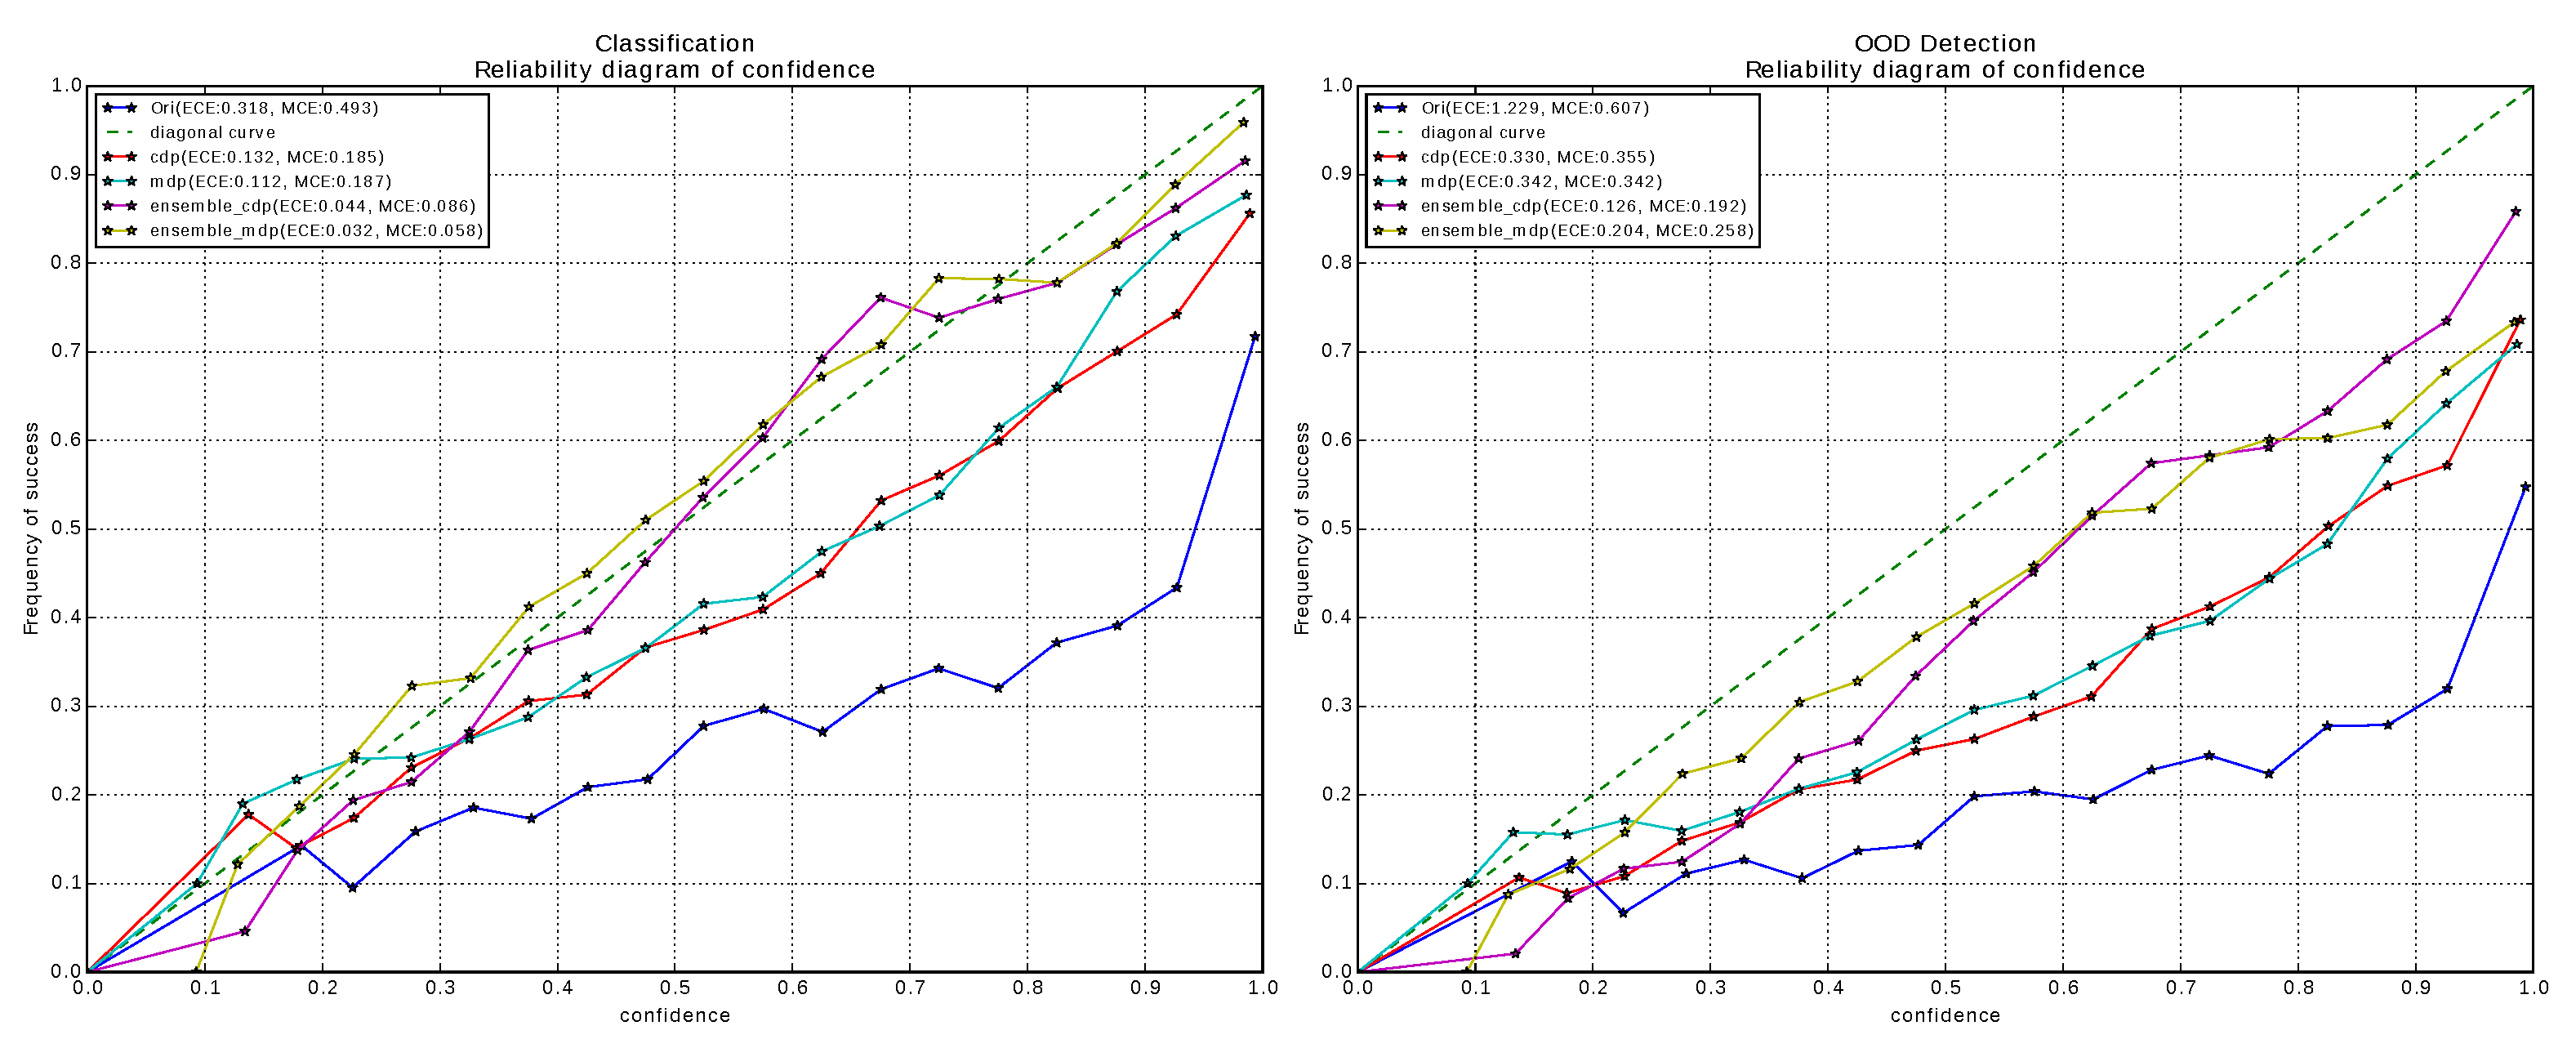
\includegraphics[height=5cm, width=16.5cm]{uncertainty_estimation/reliability_seed3_ensemble_}
		\caption{Calibration curve for ori, cdp, mdp, ensemble of cdp, ensemble of mdp from one of three runs.}		
		\label{exp2_reliability}
	\end{center}
\end{figure}

\begin{figure}[H]
	\begin{center}
		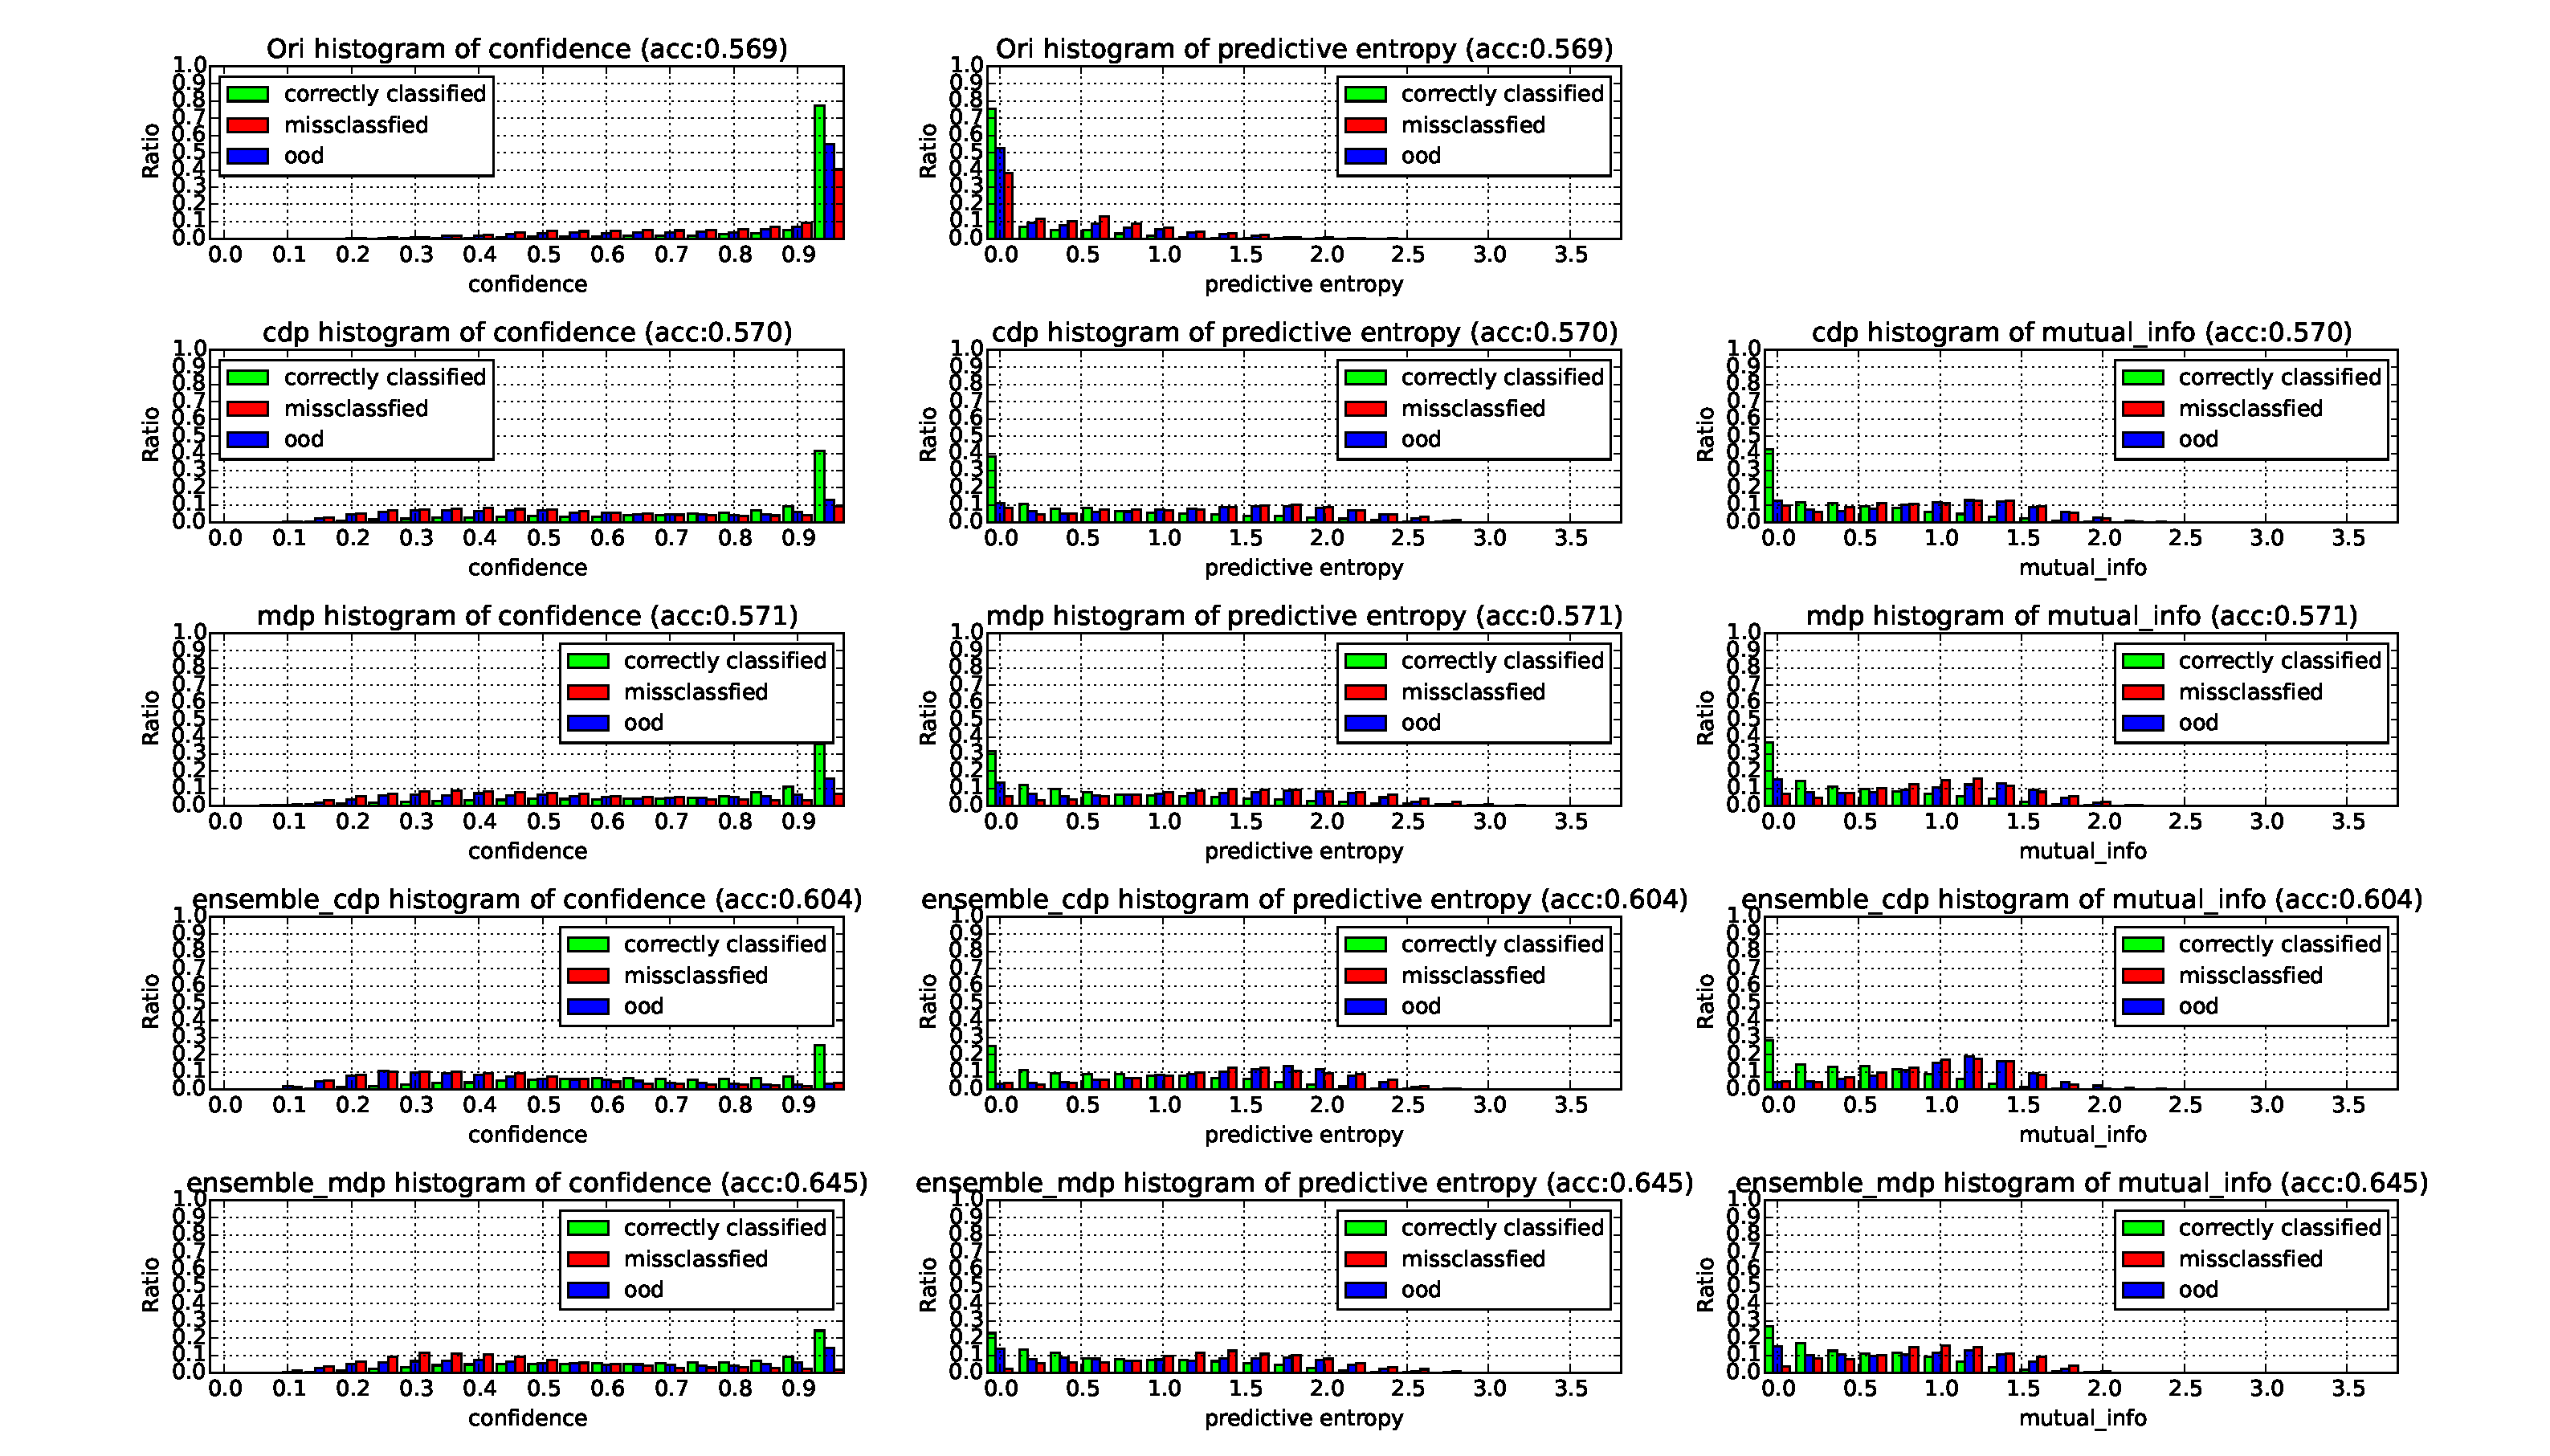
\includegraphics[height=12cm, width=16cm]{uncertainty_estimation/hist_seed3_ensemble}
		\caption{Uncertainty histograms of confidence, predictive entropy, mutual information for ori, cdp, mdp, ensemble of cdp, ensemble of mdp from one of three runs.}		
		\label{exp2_histo}
	\end{center}
\end{figure}

When it comes to the separability metrics in figure \ref{exp2_roc_pr}, as stated before, we measure separability between correct prediction and miss-classification (on the left) and that between correct prediction and OOD prediction (on the right). On separability between correction prediction and miss-classification, cdp, mdp and their ensemble version can improve the results compared with original version in both ROC curve and PR curve on the left. On the other hand, the improvements on separability between correct prediction and OOD data are more obvious on the right. However, as observed before, the ensemble of mdp does not work well with OOD data, which can be observe with this metrics. We can know more from the curves that the worse performance with OOD data in mdp is enlarged by building ensemble of it.    

\begin{figure}[h!]
	\begin{center}
		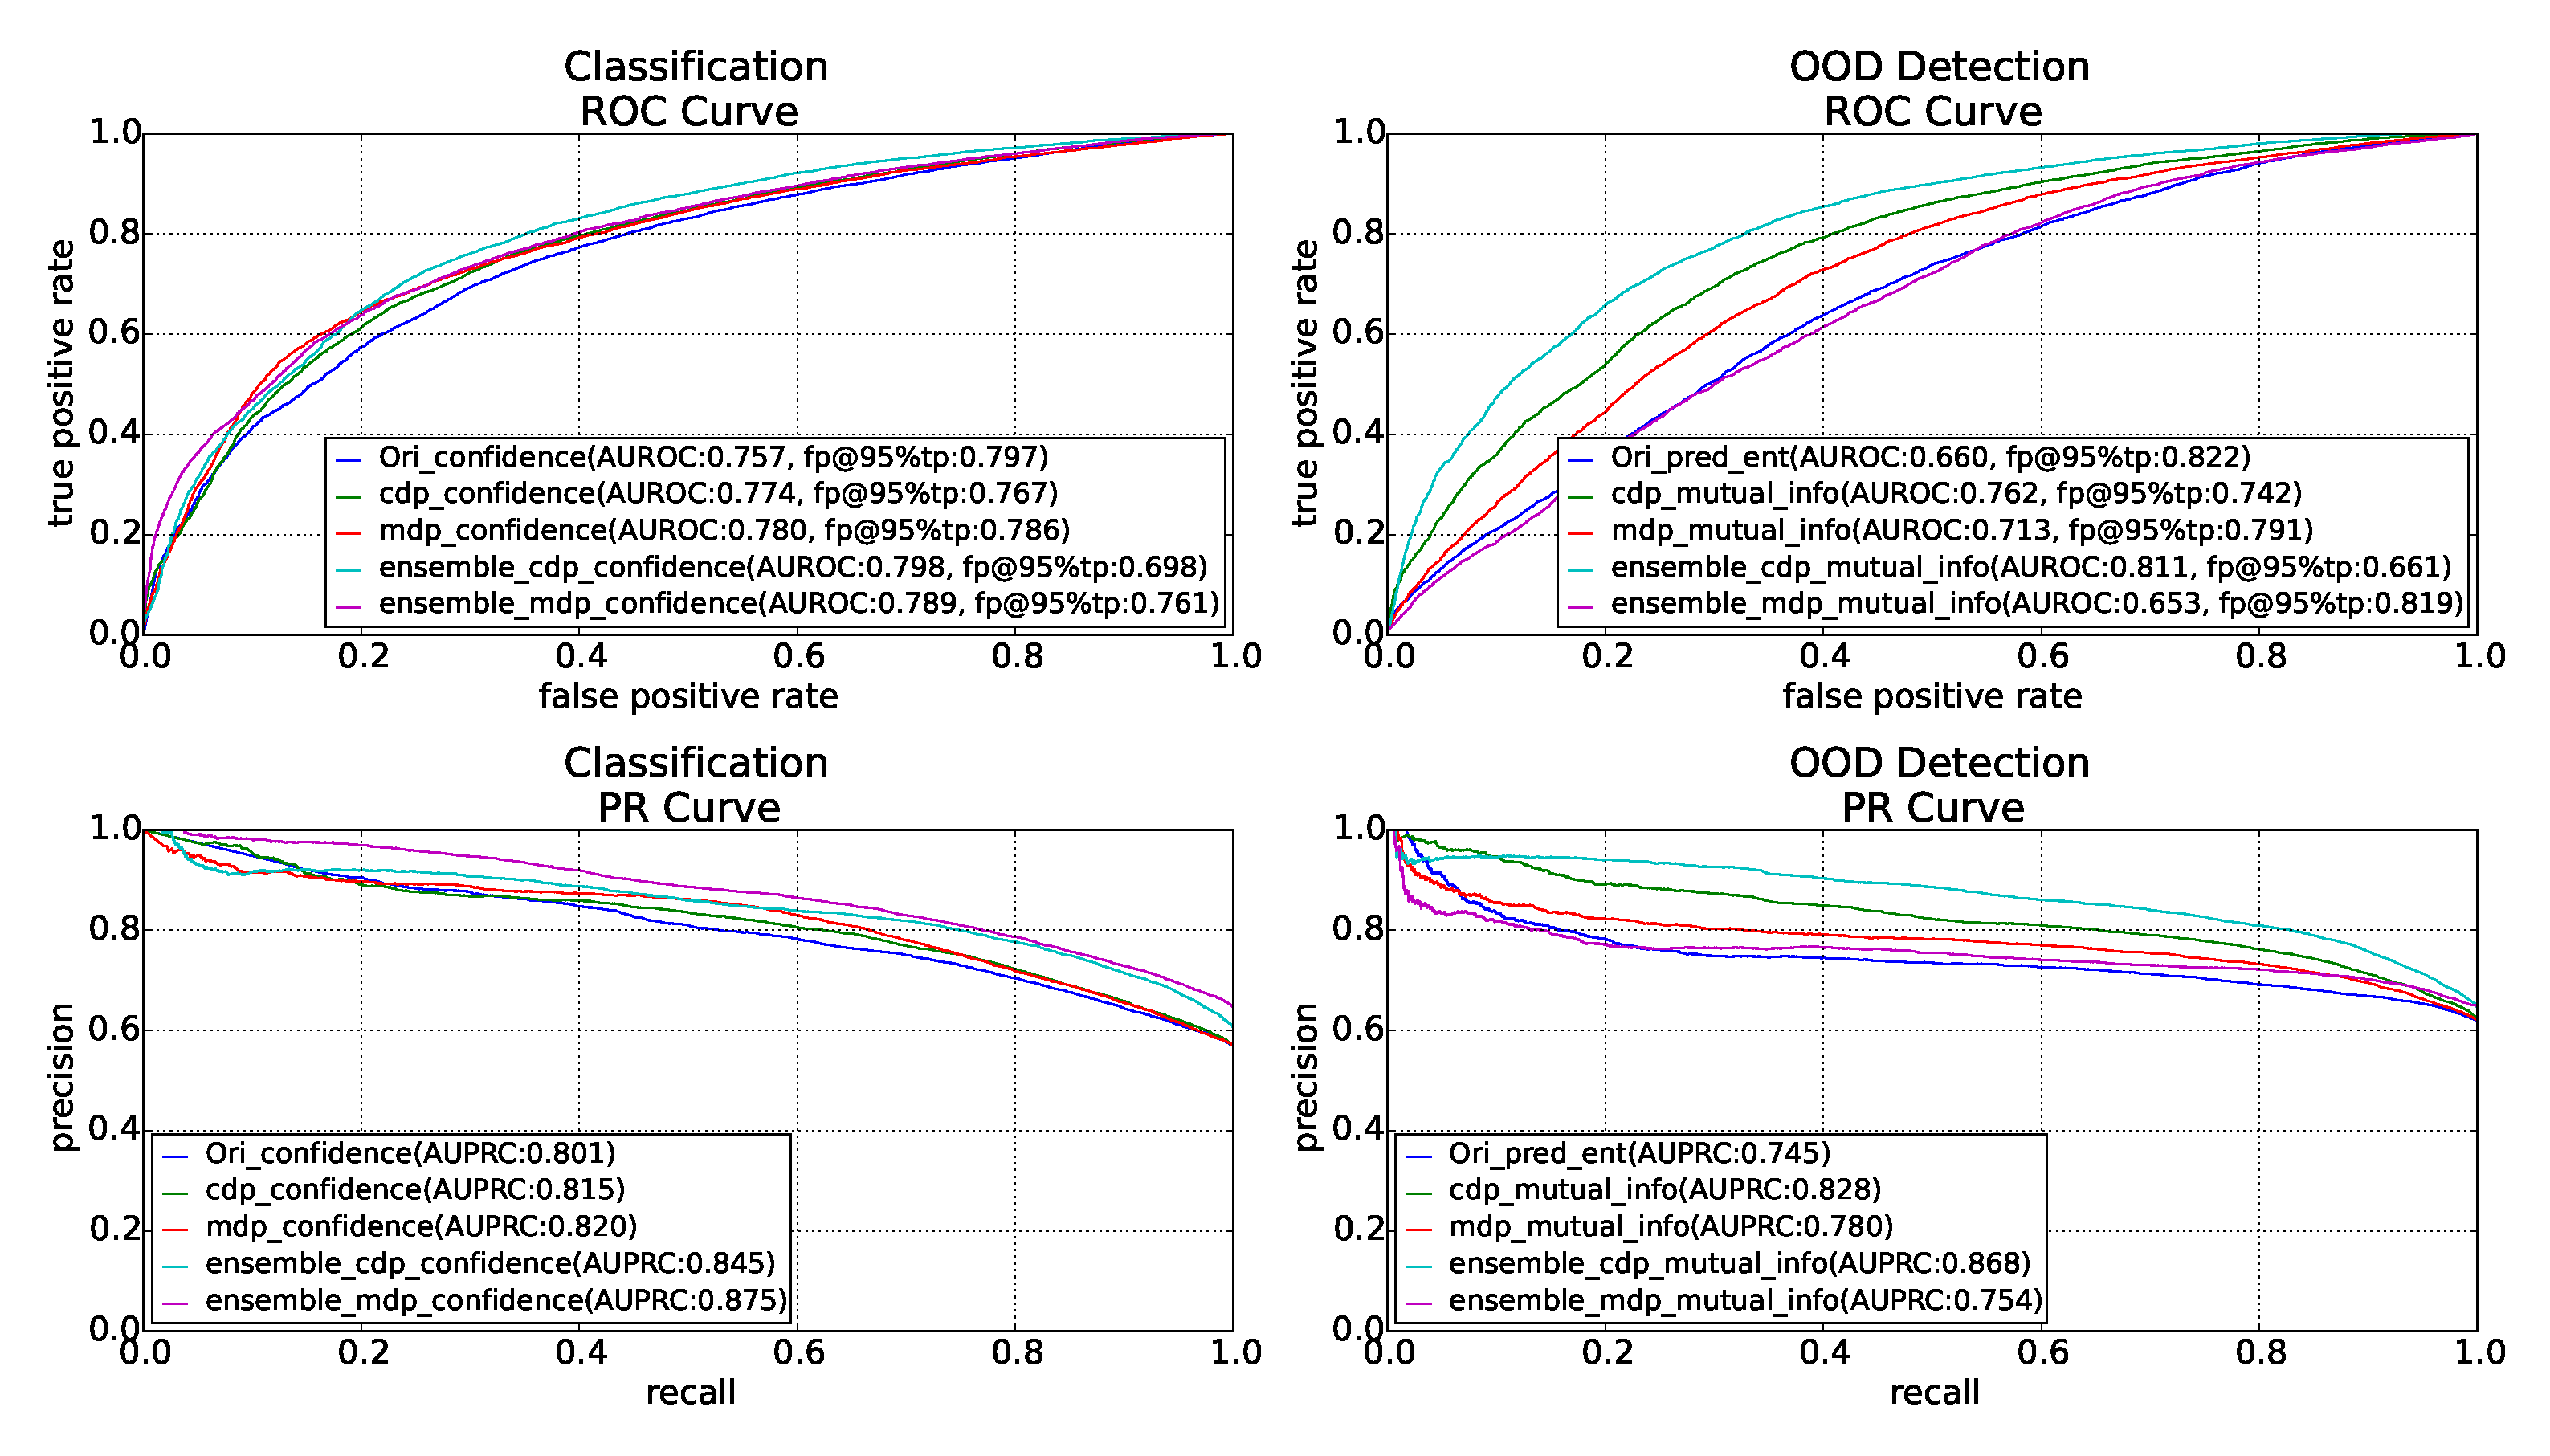
\includegraphics[height=9cm, width=16cm]{uncertainty_estimation/roc_pr_seed3_ensemble}
		\caption{ROC and PR curve of ori, cdp, mdp, ensemble of cdp, ensemble of one of three runs.}		
		\label{exp2_roc_pr}
	\end{center} 
\end{figure}

Before we only show the visual metrics for evaluation, it's better to quantify the performance quantitatively. We adopt different aforementioned metrics to achieve this which are presented in the following table \ref{table:compareWithEnsemble}. In order to exclude the influence of random initialization, we train three models of different random seeds and report the mean and standard deviation for each metric. We can see the improvements by cdp, mdp and their ensemble versions along all the metrics. The phenomenon that mdp does not work well with OOD and this effect enlarged by ensemble is also expressed in the table. Based on these experiment results, we can draw the conclusion that, concrete dropout and multiple dropout can improve both accuracy and calibration performance compared with original ResNet50. While the ensemble of concrete dropout and multiple dropout work even better without OOD data, the ensemble of multiple dropout work worse than that of concrete dropout when considering OOD data in this work. When comparing concrete dropout and multiple dropout, concrete dropout is more robust than multiple dropout because the latter one does not work well with OOD data.

\begin{table}[H]
	\centering
	\caption{Quantitative results of acc, bs, nll, ece, mce, auroc, aupr averaged from 3 different random seeds}
	\begin{tabular}{|l|l|l|l|}
		\hline
		& accuracy$ \boldsymbol\uparrow$     & brier\_score $ \boldsymbol \downarrow$& \begin{tabular}[c]{@{}l@{}}negative\\ log \\ likelihood $ \boldsymbol\downarrow$\end{tabular} \\ \hline
		ori           & 0.568$\pm$0.008 & 0.722$\pm$0.019 & 3.242$\pm$0.340                                                         \\ \hline
		cdp           & 0.577$\pm$0.008 & 0.594$\pm$0.013 & 2.088$\pm$0.181                                                         \\ \hline
		mdp           & 0.599$\pm$0.023 & 0.566$\pm$0.020 & 1.940$\pm$0.064                                                         \\ \hline
		emsemble\_cdp & 0.604        & 0.534        & 1.452                                                                \\ \hline
		emsemble\_mdp & 0.645        & 0.496        & 1.389                                                                \\ \hline
	\end{tabular}
\label{table:compareWithEnsemble}
\end{table}

\begin{table}[H]
	\centering
	% \caption{results of ece, mce, auroc, aupr}
	\begin{tabular}{|l|l|l|l|l|}
		\hline
		& \begin{tabular}[c]{@{}l@{}}expected\\ calibration\\ error(w/o. OOD/\\ w. OOD)$ \boldsymbol\downarrow$\end{tabular} & \begin{tabular}[c]{@{}l@{}}maximal\\ calibration\\ error(w/o. OOD/\\ w. OOD)$ \boldsymbol\downarrow$\end{tabular} & \begin{tabular}[c]{@{}l@{}}area under\\ ROC\\ (vs. Miss-\\ classified/\\ vs. OOD)$ \boldsymbol\uparrow$\end{tabular} & \begin{tabular}[c]{@{}l@{}}area under\\ PR curve\\ (vs. Miss-\\ classified/\\ vs. OOD)$ \boldsymbol\uparrow$\end{tabular} \\ \hline
		ori           & \begin{tabular}[c]{@{}l@{}}0.304$\pm$0.016 /\\ 0.633$\pm$0.065\end{tabular}                      & \begin{tabular}[c]{@{}l@{}}0.461$\pm$0.027 /\\ 0.362$\pm$0.025\end{tabular}                     & \begin{tabular}[c]{@{}l@{}}0.750$\pm$0.007 /\\ 0.664$\pm$0.011\end{tabular}           & \begin{tabular}[c]{@{}l@{}}0.802$\pm$0.008 /\\ 0.751$\pm$0.018\end{tabular}                \\ \hline
		cdp           & \begin{tabular}[c]{@{}l@{}}0.124$\pm$0.023/\\ 0.288$\pm$0.048\end{tabular}                         & \begin{tabular}[c]{@{}l@{}}0.206$\pm$0.015/ \\ 0.374$\pm$0.018\end{tabular}                     & \begin{tabular}[c]{@{}l@{}}0.775$\pm$0.008/ \\ 0.783$\pm$0.022\end{tabular}           & \begin{tabular}[c]{@{}l@{}}0.825$\pm$0.007/ \\ 0.850$\pm$0.022\end{tabular}                \\ \hline
		mdp           & \begin{tabular}[c]{@{}l@{}}0.114$\pm$0.012/ \\ 0.383$\pm$0.046\end{tabular}                      & \begin{tabular}[c]{@{}l@{}}0.199$\pm$0.016/ \\ 0.367$\pm$0.023\end{tabular}                     & \begin{tabular}[c]{@{}l@{}}0.780$\pm$0.011/ \\ 0.709$\pm$0.004\end{tabular}           & \begin{tabular}[c]{@{}l@{}}0.838$\pm$0.013/ \\ 0.788$\pm$0.006\end{tabular}                \\ \hline
		emsemble\_cdp & \begin{tabular}[c]{@{}l@{}}0.044/\\0.042 \end{tabular} 
		 &  \begin{tabular}[c]{@{}l@{}}0.086/\\0.093 \end{tabular}                                                                                    & \begin{tabular}[c]{@{}l@{}}0.798/\\0.811  \end{tabular}                                                                           & \begin{tabular}[c]{@{}l@{}}0.845/\\0.868  \end{tabular}                                                                                \\ \hline
		emsemble\_mdp & \begin{tabular}[c]{@{}l@{}}0.032/\\0.170 \end{tabular}                                                                                       & \begin{tabular}[c]{@{}l@{}}0.058/\\0.227  \end{tabular}                                                                                     & \begin{tabular}[c]{@{}l@{}}0.789/\\0.653 \end{tabular}                                                                            & \begin{tabular}[c]{@{}l@{}}0.875/\\0.754  \end{tabular}                                                                                \\ \hline
	\end{tabular}
\end{table}	

\newpage
\subsubsection{Comparison with Laplace approximation}
Because Laplace approximation requires only MAP point estimate of model parameter. Therefore we take the already trained model of different approaches as our MAP point estimate and compute the approximation of Kronecker factors with half of training set. We set the scale parameter of Kronecker factors $\sqrt{N}$ as $1$ and dump factor $\sqrt{\tau}$ as $15$ in equation \ref{mvg_prior} based on grid search on the validation set.   

In the following figures, we show the histograms, calibration curves, ROC curve and PR curve of cdp, mdp and their Laplace approximation versions. We can see that the Laplace approximation can achieve similar results as the cdp or mdp do in uncertainty histograms, calibration curves as well as ROC curve and PR curve. The histograms of different uncertainty measure show similar trend as before. 

If we compare the Laplace approximation between cdp and mdp, we can see that the result of Laplace approximation is similar to the their dropout versions. This can be observed through that the percentage of OOD prediction with high confidence of Laplace approximation for network trained with mdp is higher than that of Laplace approximation for network trained with cdp in the histogram. Besides, in ROC curve/PR curve on correct prediction vs. OOD data prediction of mdp and cdp, the area under curve of Laplace approximation of mdp is obviously lower than that of cdp. This phenomenon also exists in the histogram and ROC as well as PR curve of mdp and cdp. In the table of quantitative results (cf. \ref{table:lap}), the quantities of different metrics corresponding to the visual metrics. To summarize this, although Laplace can achieve similar results as concrete dropout and multiple dropout do, their performance is highly related to the point estimate of parameter obtained during training.

\begin{figure}[H]
	\begin{center}
		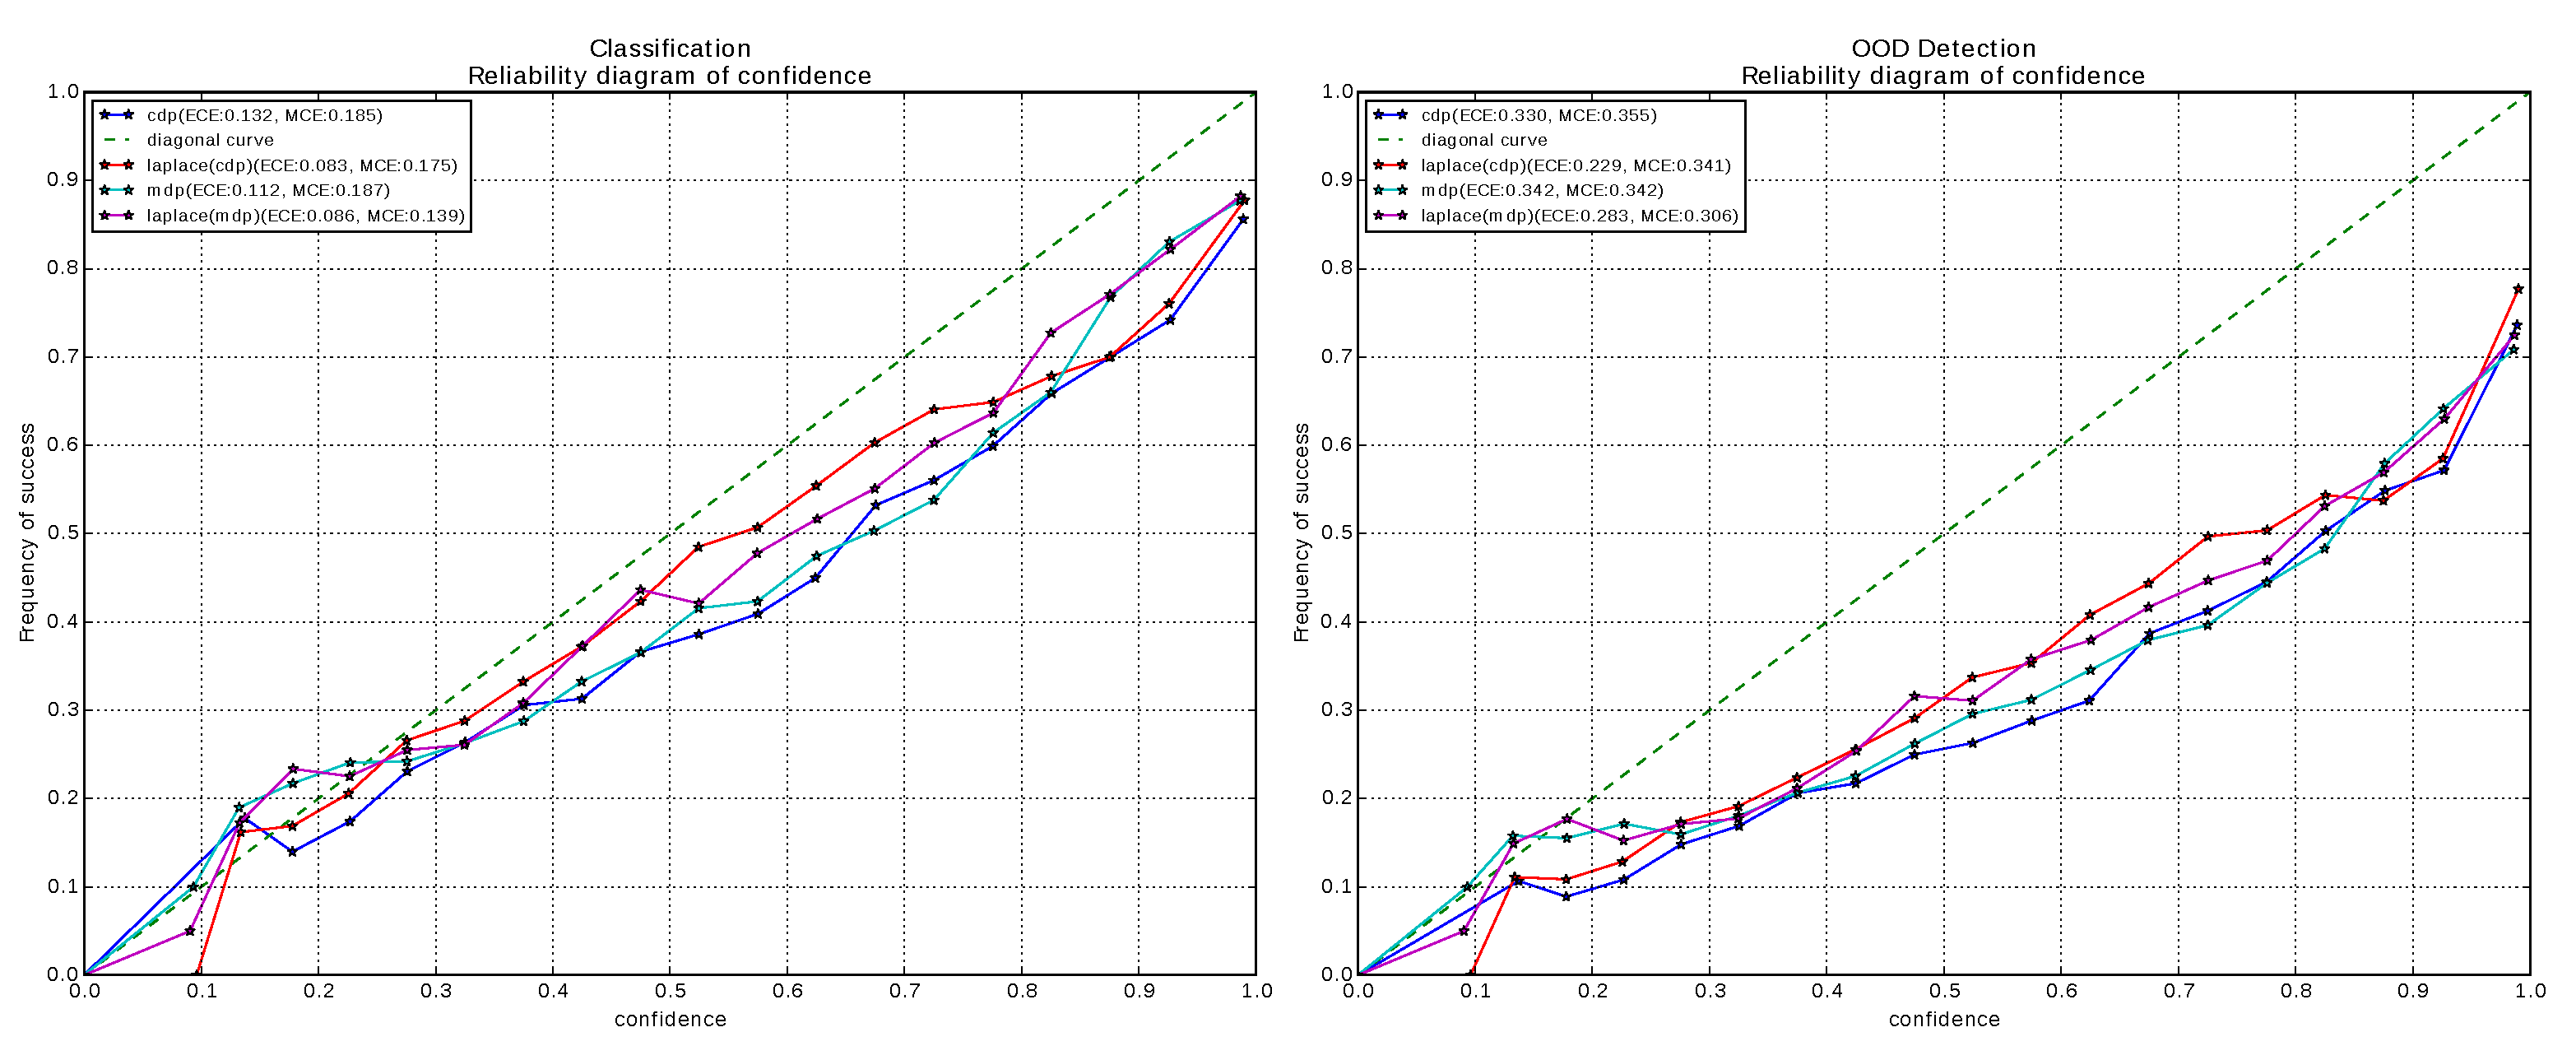
\includegraphics[height=5cm, width=16.5cm]{uncertainty_estimation/laplace/reliabilty_seed3_}
		\caption{Calibration curve of cdp, mdp and their Laplace approximation versions from one of three runs.}		
		\label{lap_calibration}
	\end{center}
\end{figure}

\begin{figure}[h!]		
	\centering
	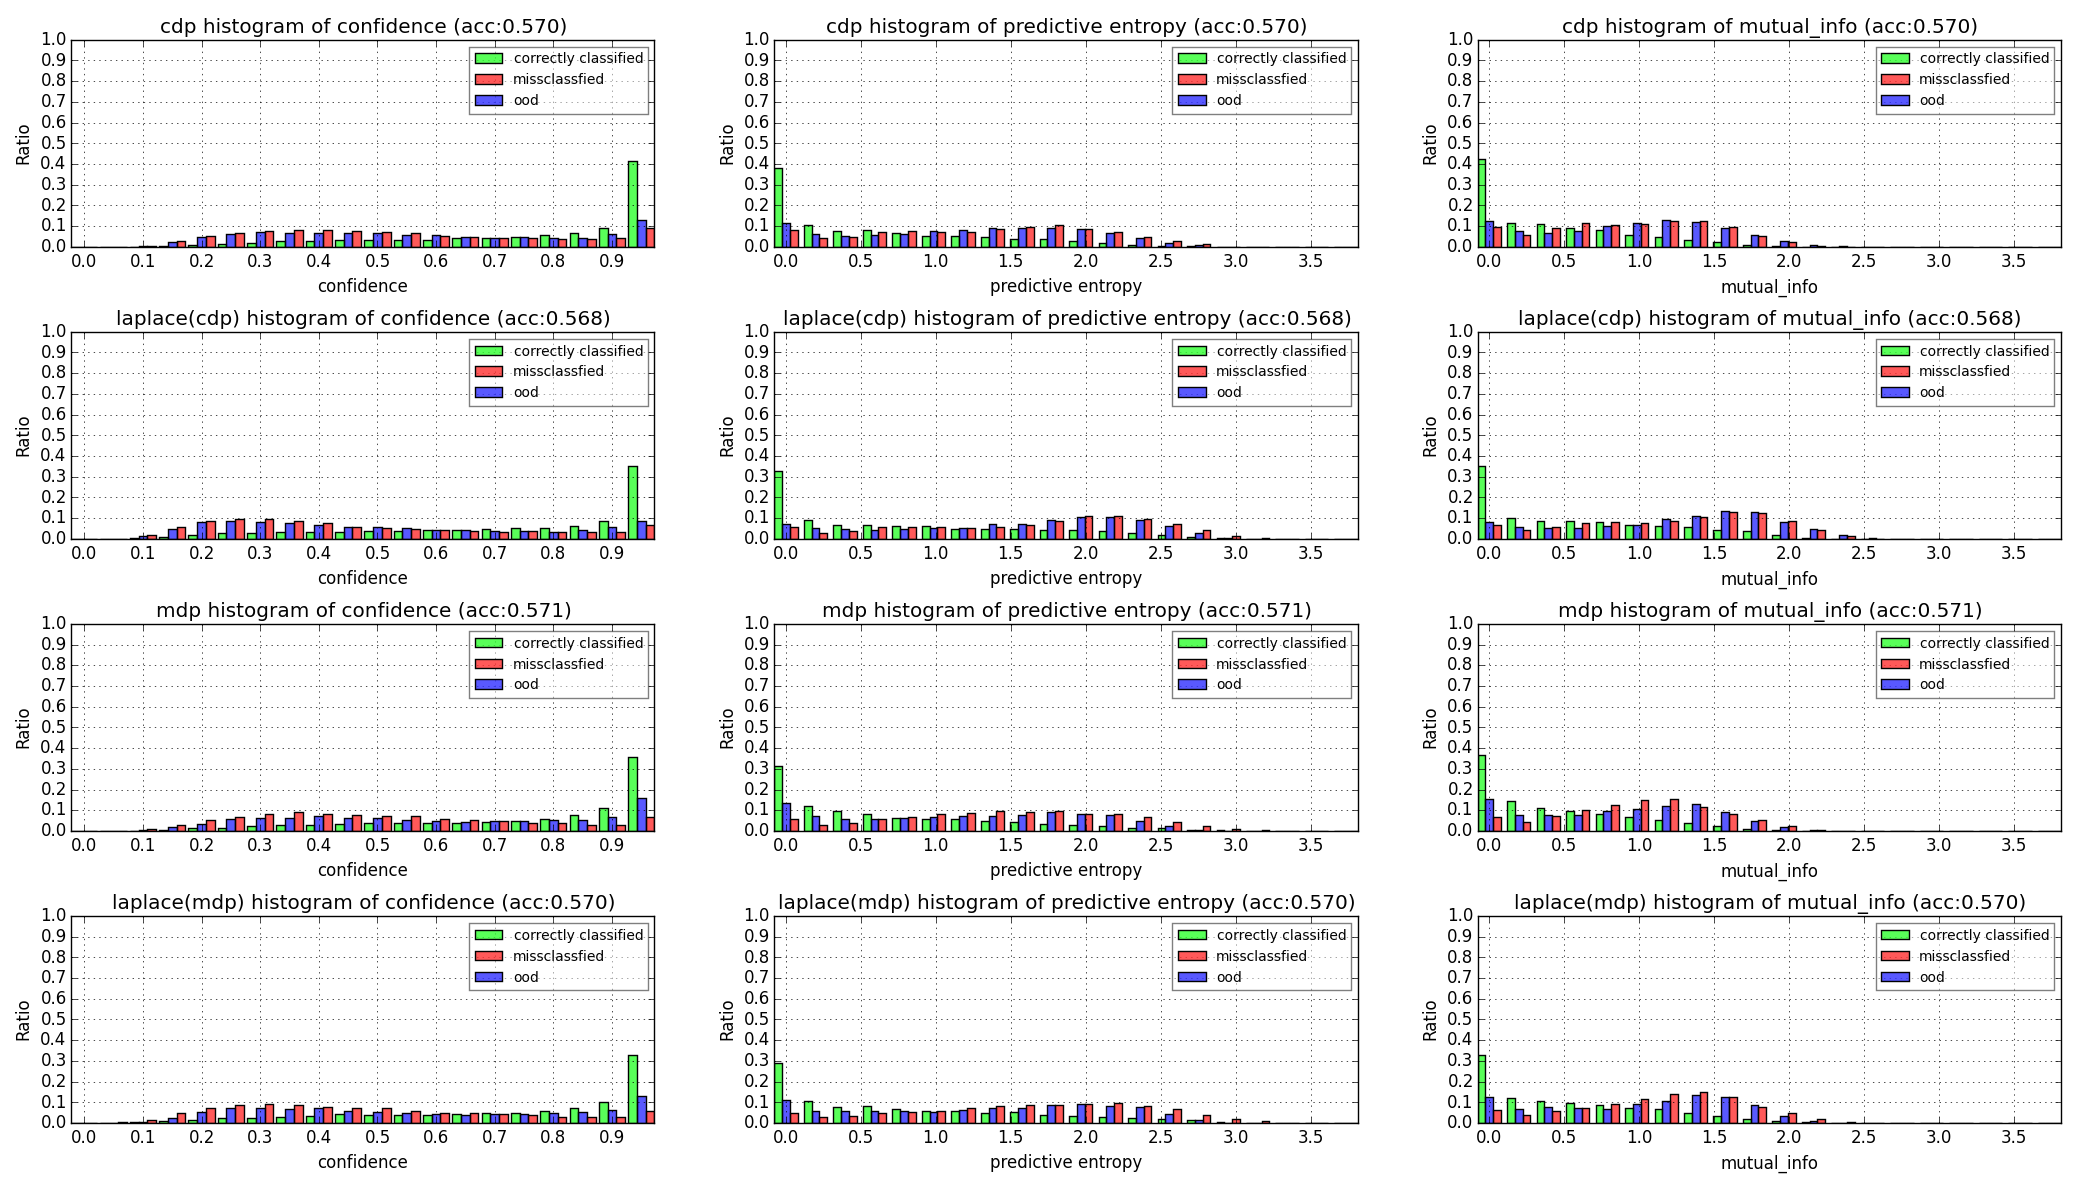
\includegraphics[height=9cm, width=16cm]{uncertainty_estimation/laplace/histo_ood_seed3}
	\caption{Uncertainty histogram of cdp, mdp and their Laplace approximation versions with confidence, predictive entropy and mutual information as uncertainty measure in one of three runs.}
	\label{figure:lap_hist}	
\end{figure}


\begin{figure}[H]
	\begin{center}
		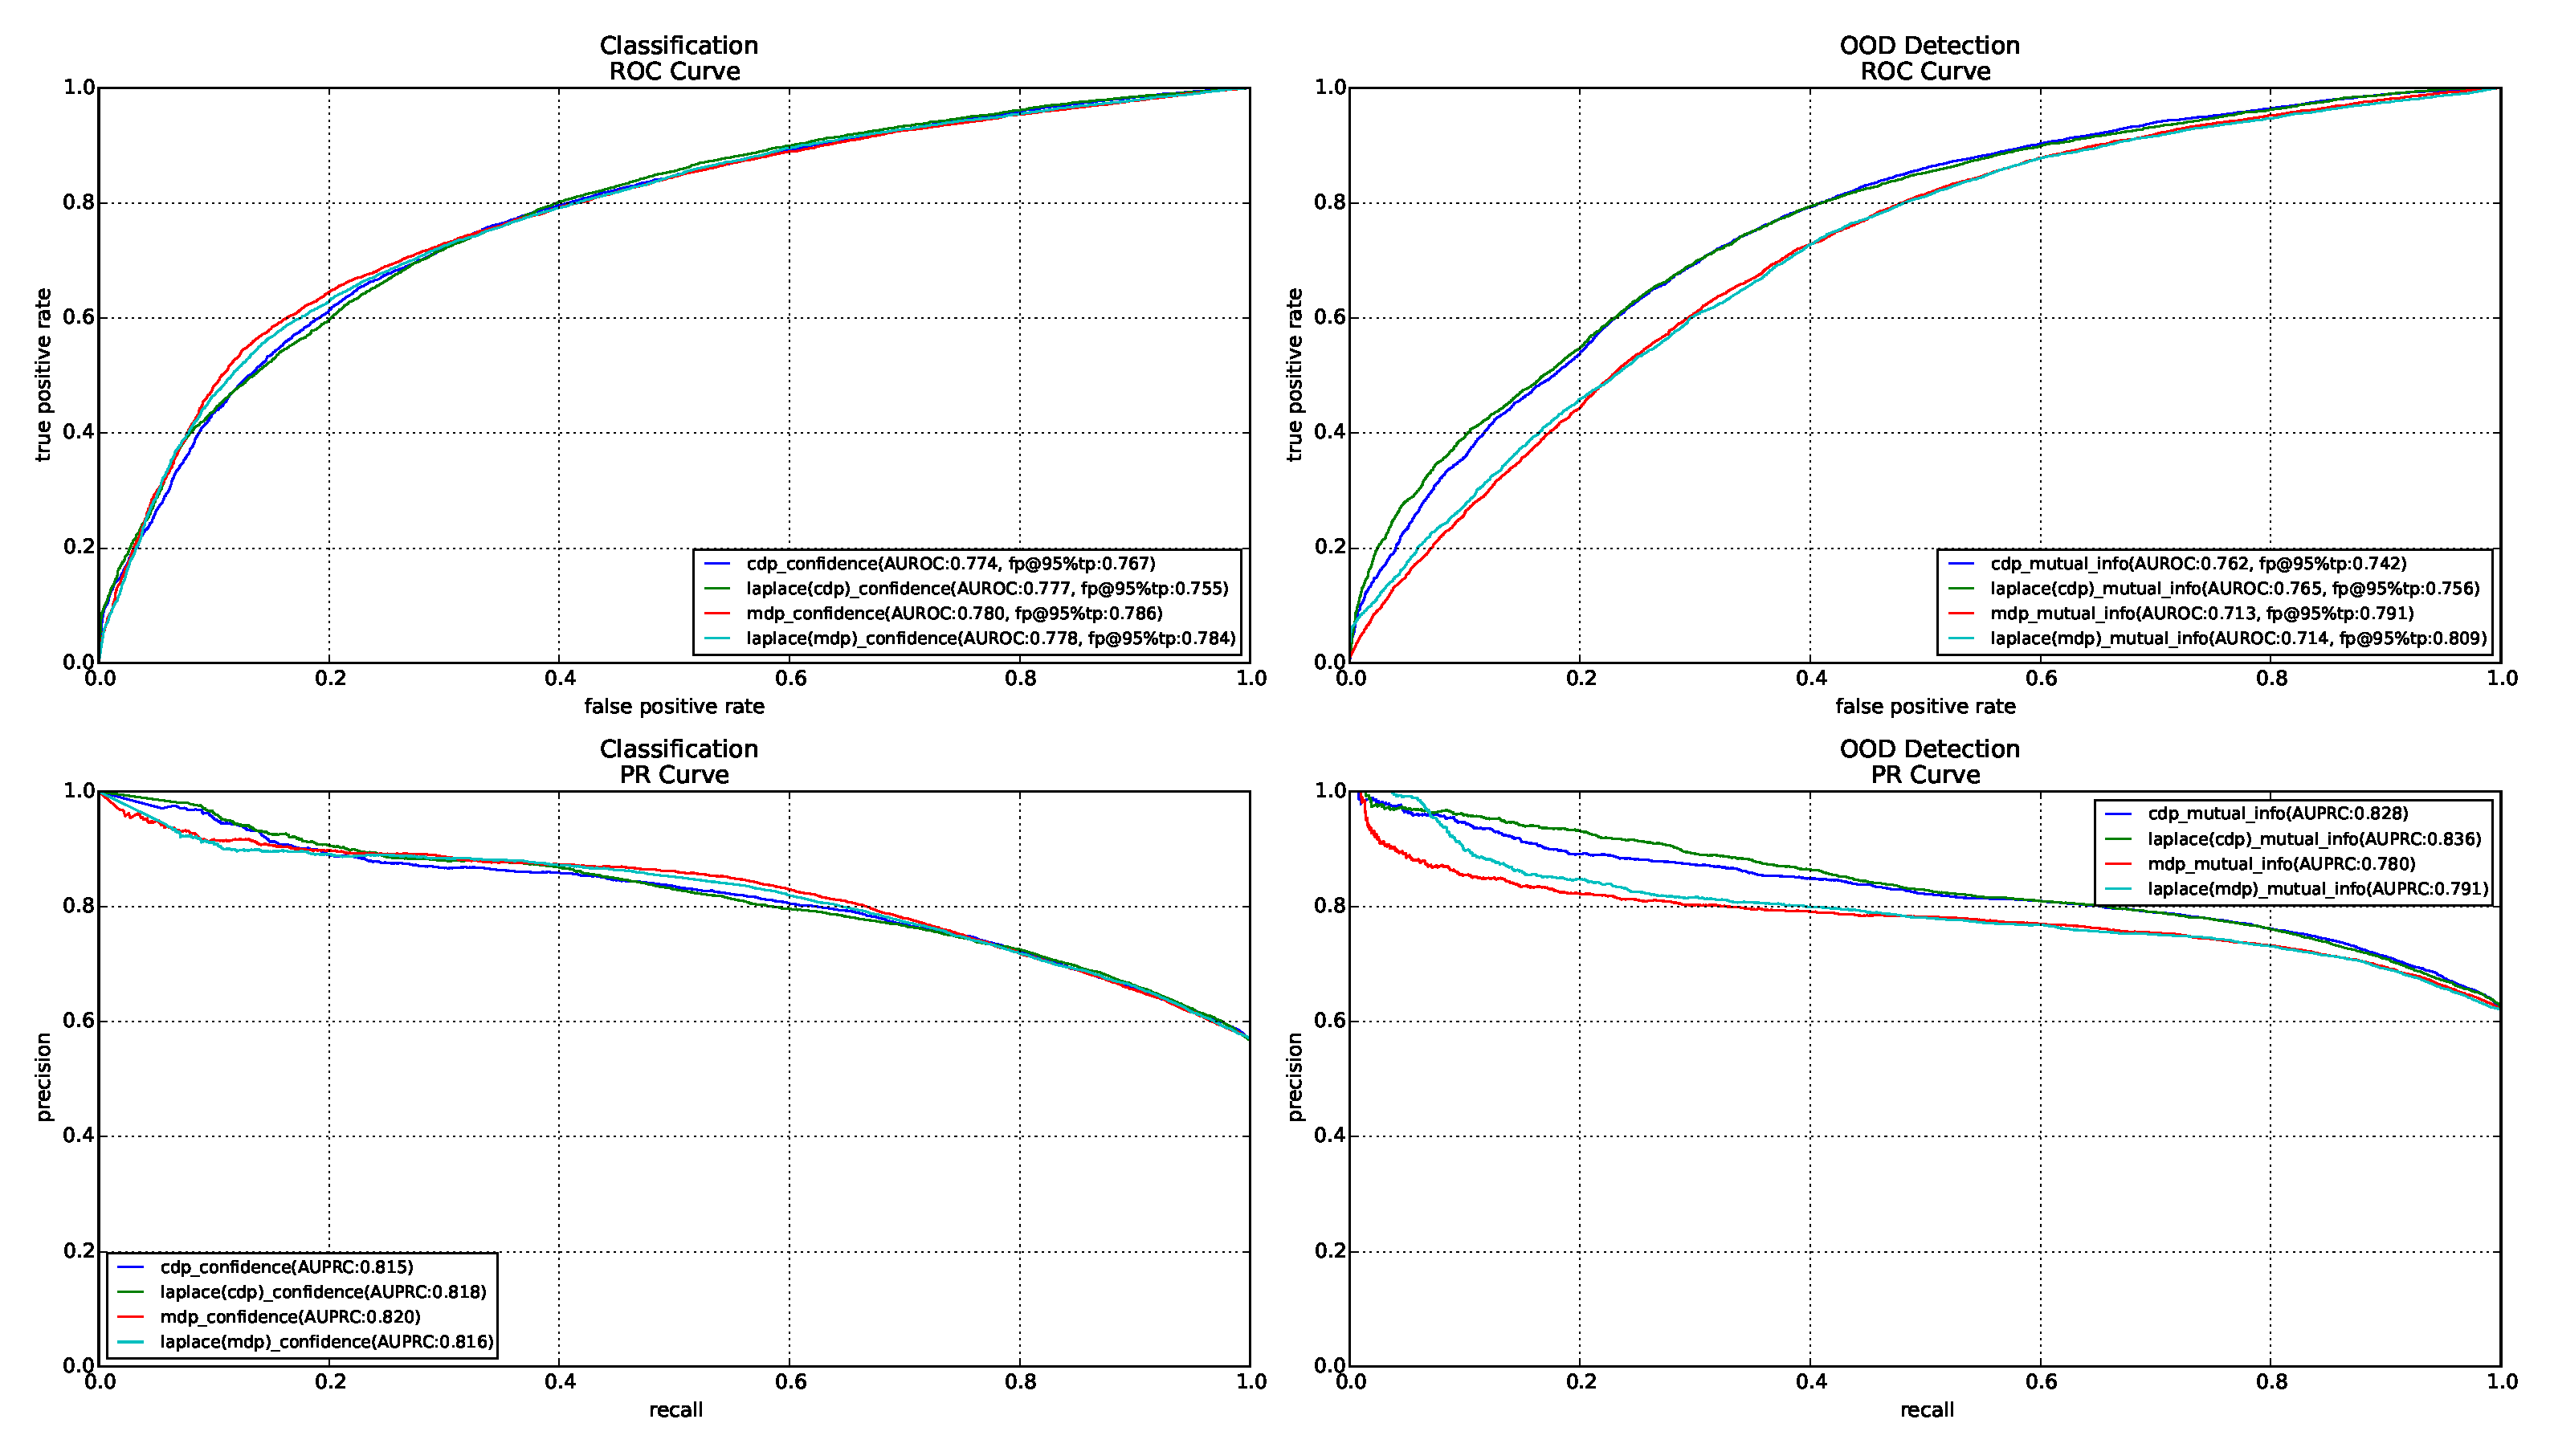
\includegraphics[height=9cm, width=16cm]{uncertainty_estimation/laplace/roc_pr_seed3}
		\caption{ROC and PR curve of cdp, mdp and their Laplace approximation versions from one of three runs.}		
		\label{lap_roc_pr}
	\end{center}
\end{figure}

\begin{table}[H]
	\centering
	\label{table:lap}
	\caption{Quantitative results of acc, bs, nll, ece, mce, auroc, aupr averaged from 3 different random seeds}
	\begin{tabular}{|l|l|l|l|}
		\hline
		& accuracy  $\boldsymbol \uparrow$                                                            & brier score $\boldsymbol \downarrow$                                                           & \begin{tabular}[c]{@{}l@{}}negative \\ log\\ likelihood $\boldsymbol \downarrow$\end{tabular}  \\ \hline
		cdp          & 
		\begin{tabular}[c]{@{}l@{}}0.577$\pm$0.008\end{tabular} & 
		\begin{tabular}[c]{@{}l@{}}0.594$\pm$0.013\end{tabular} & \begin{tabular}[c]{@{}l@{}}2.088$\pm$0.181\end{tabular} \\ \hline
		
		laplace\_cdp & 
		\begin{tabular}[c]{@{}l@{}}0.576$\pm$0.009\end{tabular}    & \begin{tabular}[c]{@{}l@{}}0.602$\pm$0.011\end{tabular} & \begin{tabular}[c]{@{}l@{}}2.322$\pm$0.350\end{tabular} \\ \hline
		
		mdp          & 
		\begin{tabular}[c]{@{}l@{}}0.599$\pm$0.023\end{tabular} & \begin{tabular}[c]{@{}l@{}}0.566$\pm$0.020\end{tabular} & \begin{tabular}[c]{@{}l@{}}1.940$\pm$0.064\end{tabular} \\ \hline
		laplace\_mdp & 		\begin{tabular}[c]{@{}l@{}}0.598$\pm$0.024\end{tabular} & \begin{tabular}[c]{@{}l@{}}0.567$\pm$0.018\end{tabular} & \begin{tabular}[c]{@{}l@{}}1.970$\pm$0.117\end{tabular} \\ \hline
	\end{tabular}
\end{table}
\begin{table}[H]
	\centering
	\begin{tabular}{|l|l|l|l|l|}
		\hline
		& \begin{tabular}[c]{@{}l@{}}expected\\ calibration\\ error(w/o. OOD/\\ w. OOD) $\boldsymbol \downarrow$\end{tabular} & \begin{tabular}[c]{@{}l@{}}maximal\\ calibration\\ error(w/o. OOD/\\ w. OOD)$\boldsymbol \downarrow$\end{tabular} & \begin{tabular}[c]{@{}l@{}}area under\\ ROC\\ (vs. Miss-\\ classified/\\ vs. OOD)$\boldsymbol \uparrow$\end{tabular} & \begin{tabular}[c]{@{}l@{}}area under\\ PR curve\\ (vs. Miss-\\ classified/\\ vs. OOD)$\boldsymbol \uparrow$\end{tabular} \\ \hline
		
		cdp          & \begin{tabular}[c]{@{}l@{}}0.124$\pm$0.023/ \\0.288$\pm$0.048\end{tabular}                      & \begin{tabular}[c]{@{}l@{}}0.206$\pm$0.015/ \\0.374$\pm$0.018\end{tabular}                     & \begin{tabular}[c]{@{}l@{}}0.775$\pm$0.008/ \\0.783$\pm$0.022\end{tabular}           & \begin{tabular}[c]{@{}l@{}}0.825$\pm$0.007/ \\0.850$\pm$0.022\end{tabular}                \\ \hline
		
		laplace\_cdp & \begin{tabular}[c]{@{}l@{}}0.129$\pm$0.058/ \\0.341$\pm$0.157\end{tabular}                         & \begin{tabular}[c]{@{}l@{}}0.235$\pm$0.073/ \\0.406$\pm$0.070\end{tabular}                     & \begin{tabular}[c]{@{}l@{}}0.779$\pm$0.004/ \\0.782$\pm$0.017\end{tabular}           & \begin{tabular}[c]{@{}l@{}}0.826$\pm$0.007/ \\0.849$\pm$0.016\end{tabular}                \\ \hline
		
		mdp          & \begin{tabular}[c]{@{}l@{}}0.114$\pm$0.012/ \\0.383$\pm$0.046\end{tabular}                      & \begin{tabular}[c]{@{}l@{}}0.199$\pm$0.016/ \\0.367$\pm$0.023\end{tabular}                     & \begin{tabular}[c]{@{}l@{}}0.780$\pm$0.011/ \\0.709$\pm$0.004\end{tabular}           & \begin{tabular}[c]{@{}l@{}}0.838$\pm$0.013/ \\0.788$\pm$0.006\end{tabular}                \\ \hline
		
		laplace\_mdp         & \begin{tabular}[c]{@{}l@{}} 0.104$\pm$0.018/ \\0.352$\pm$0.061\end{tabular}                      & \begin{tabular}[c]{@{}l@{}}0.179$\pm$0.029/ \\0.352$\pm$0.038\end{tabular}                     & \begin{tabular}[c]{@{}l@{}}0.776$\pm$0.012/ \\0.711$\pm$0.005\end{tabular}           & \begin{tabular}[c]{@{}l@{}}0.837$\pm$0.015/ \\0.798$\pm$0.005\end{tabular}                \\ \hline
	\end{tabular}
\end{table}
\subsubsection{Ablation study}
As we can see from the previous results, mdp can work better than cdp without considering OOD data. However, it underperforms when OOD data is included. In order to investigate the reason behind this, we have done a ablation study to check the influence of aleatoric uncertainty which comes from mainly the feature extractor part. To this end, we firstly make assumption that the feature extractor part has a dominant effect on the aleatoric uncertainty, because it's deterministic compared with the following MLP classifier. 

Considering this, we freeze the parameters of feature extractor trying to keep the dominant effect on aleatoric uncertainty fixed for different approaches and just train our probabilistic classifier which is a three-layer MLP. In the following we show the results of this ablation study with the same metrics used before. It's clear that the accuracy would drop when the feature extractor is frozen. However, we can see that mdp can have better  calibration performance than cdp and much better than original ResNet50. Regarding the separability metrics, although mdp still doesn't work better than cdp, the gap between is much smaller than the version without freezing feature extractor. These observations are expressed quantitatively in the table \ref{ab_table}. 

Based on these observations, we know that the underperformance of mdp on OOD dataset can attribute to the influence of aleatoric uncertainty. If the feature extractor is not frozen, then the aleatoric uncertainty is trained to adapt to the dataset. The problem why optimizing dropout rates for each hidden units can change the point estimate of the model parameter to have low aleatoric uncertainty for OOD data arises here. One possible reason for this could be the variance of estimation of derivatives of variational parameters is too large because of increased number of variational parameters\cite{kingma2015variational}. And the larger variances are back propagated to the feature extractor which may make the point estimate deviate from the better local minimum. One possible solution to resolve this is to sample the realization of activations of hidden units independent to each data instance, which may decrease the variance and help to improve the results. 

\begin{figure}[H]
	\begin{center}
		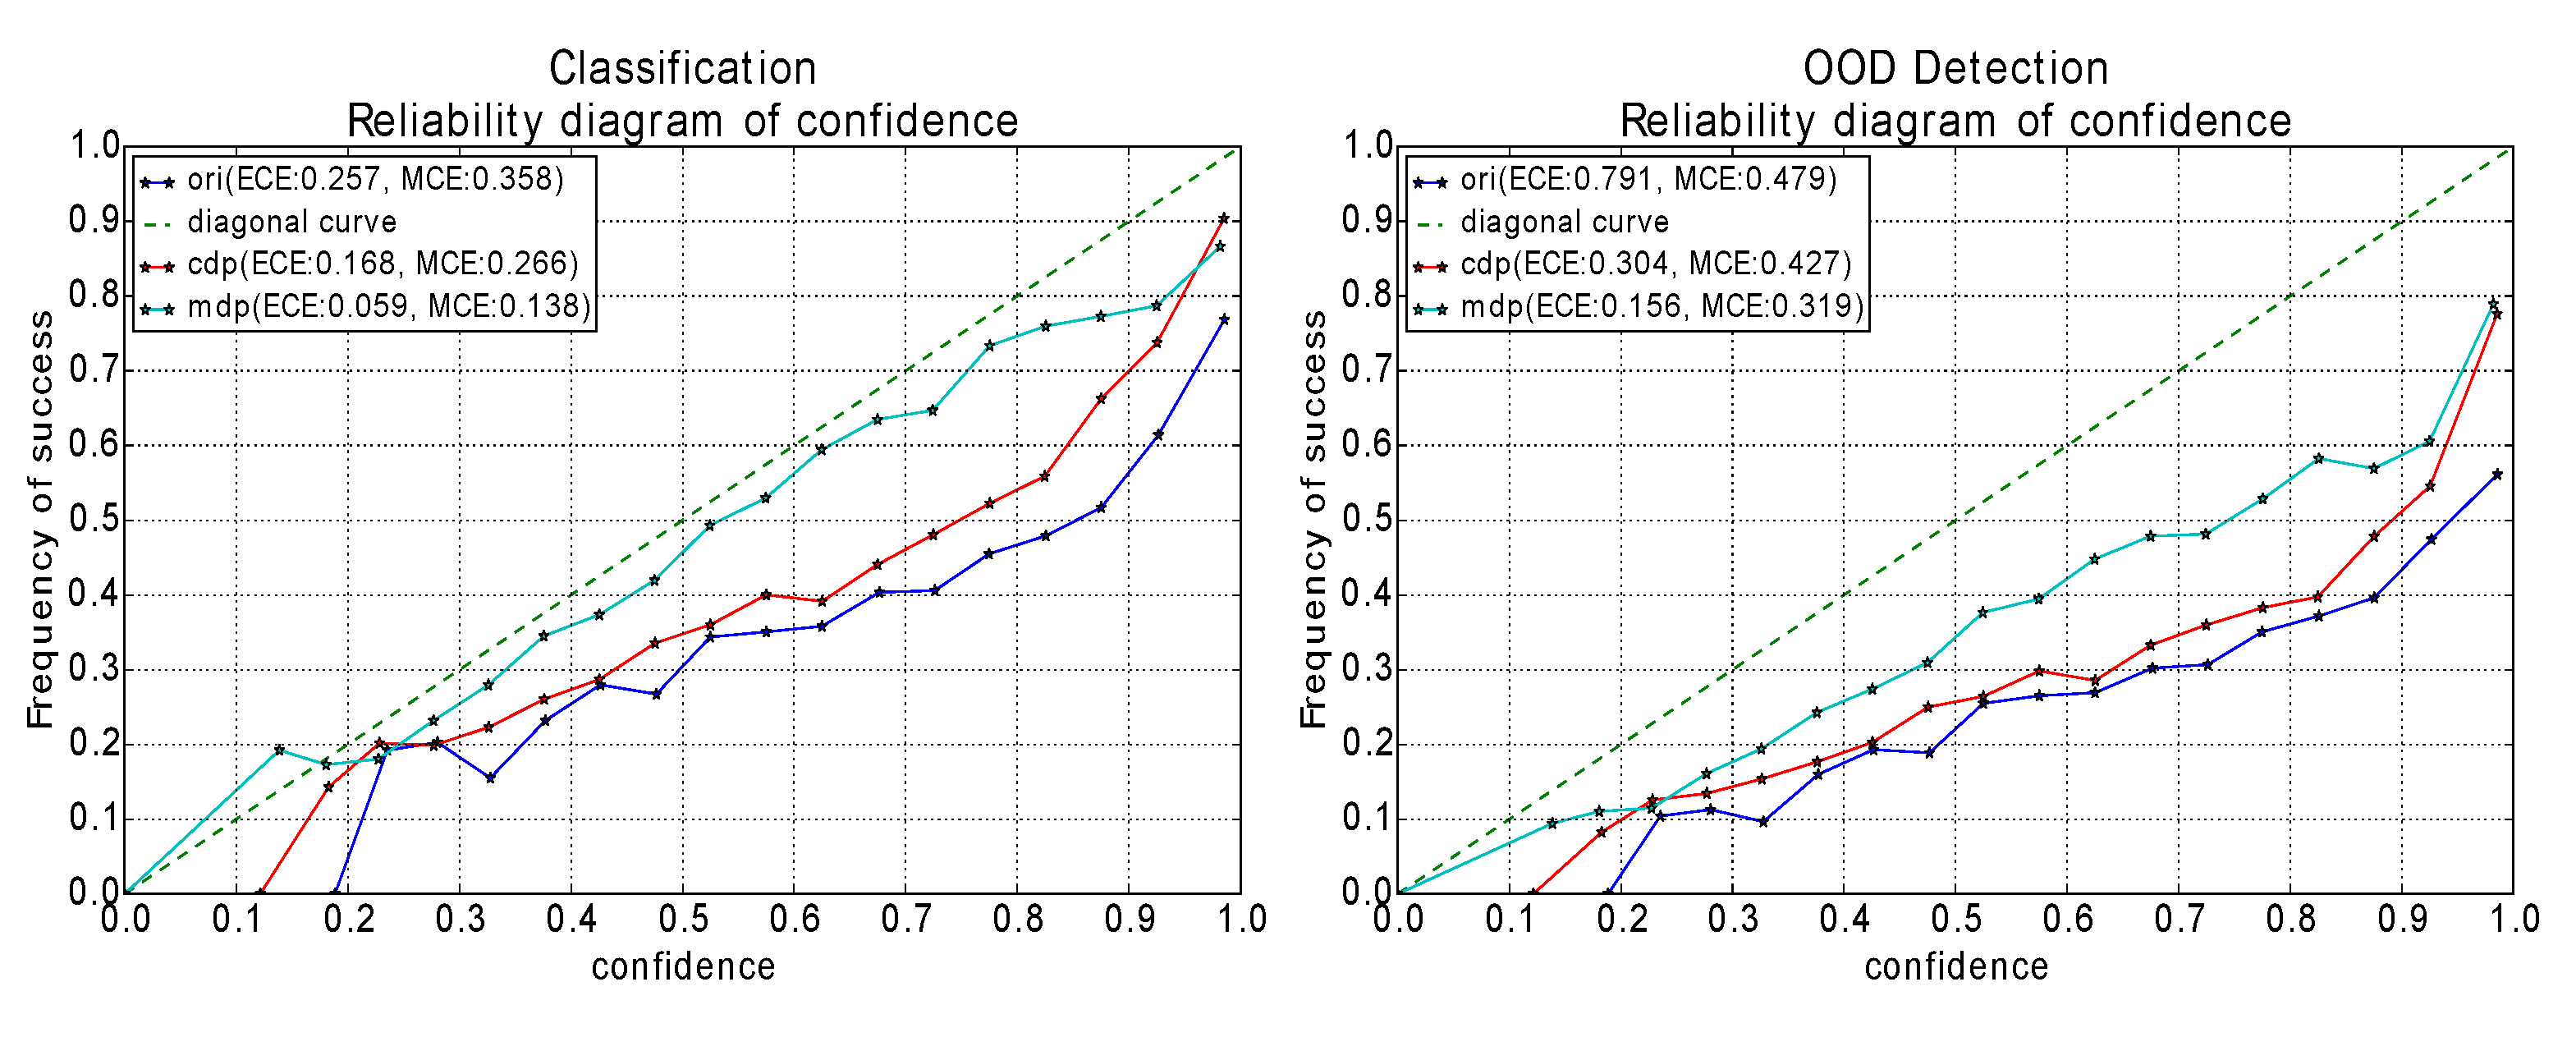
\includegraphics[height=4.5cm, width=16.5cm]{uncertainty_estimation/ablation_study/reliability_froFeat_ori_cdp_mdp_combined_seed3_.eps}
		\caption{Calibration curve of one of three runs.}		
		\label{ab_calibration}
	\end{center}
\end{figure}

\begin{figure}[H]
	\begin{center}
		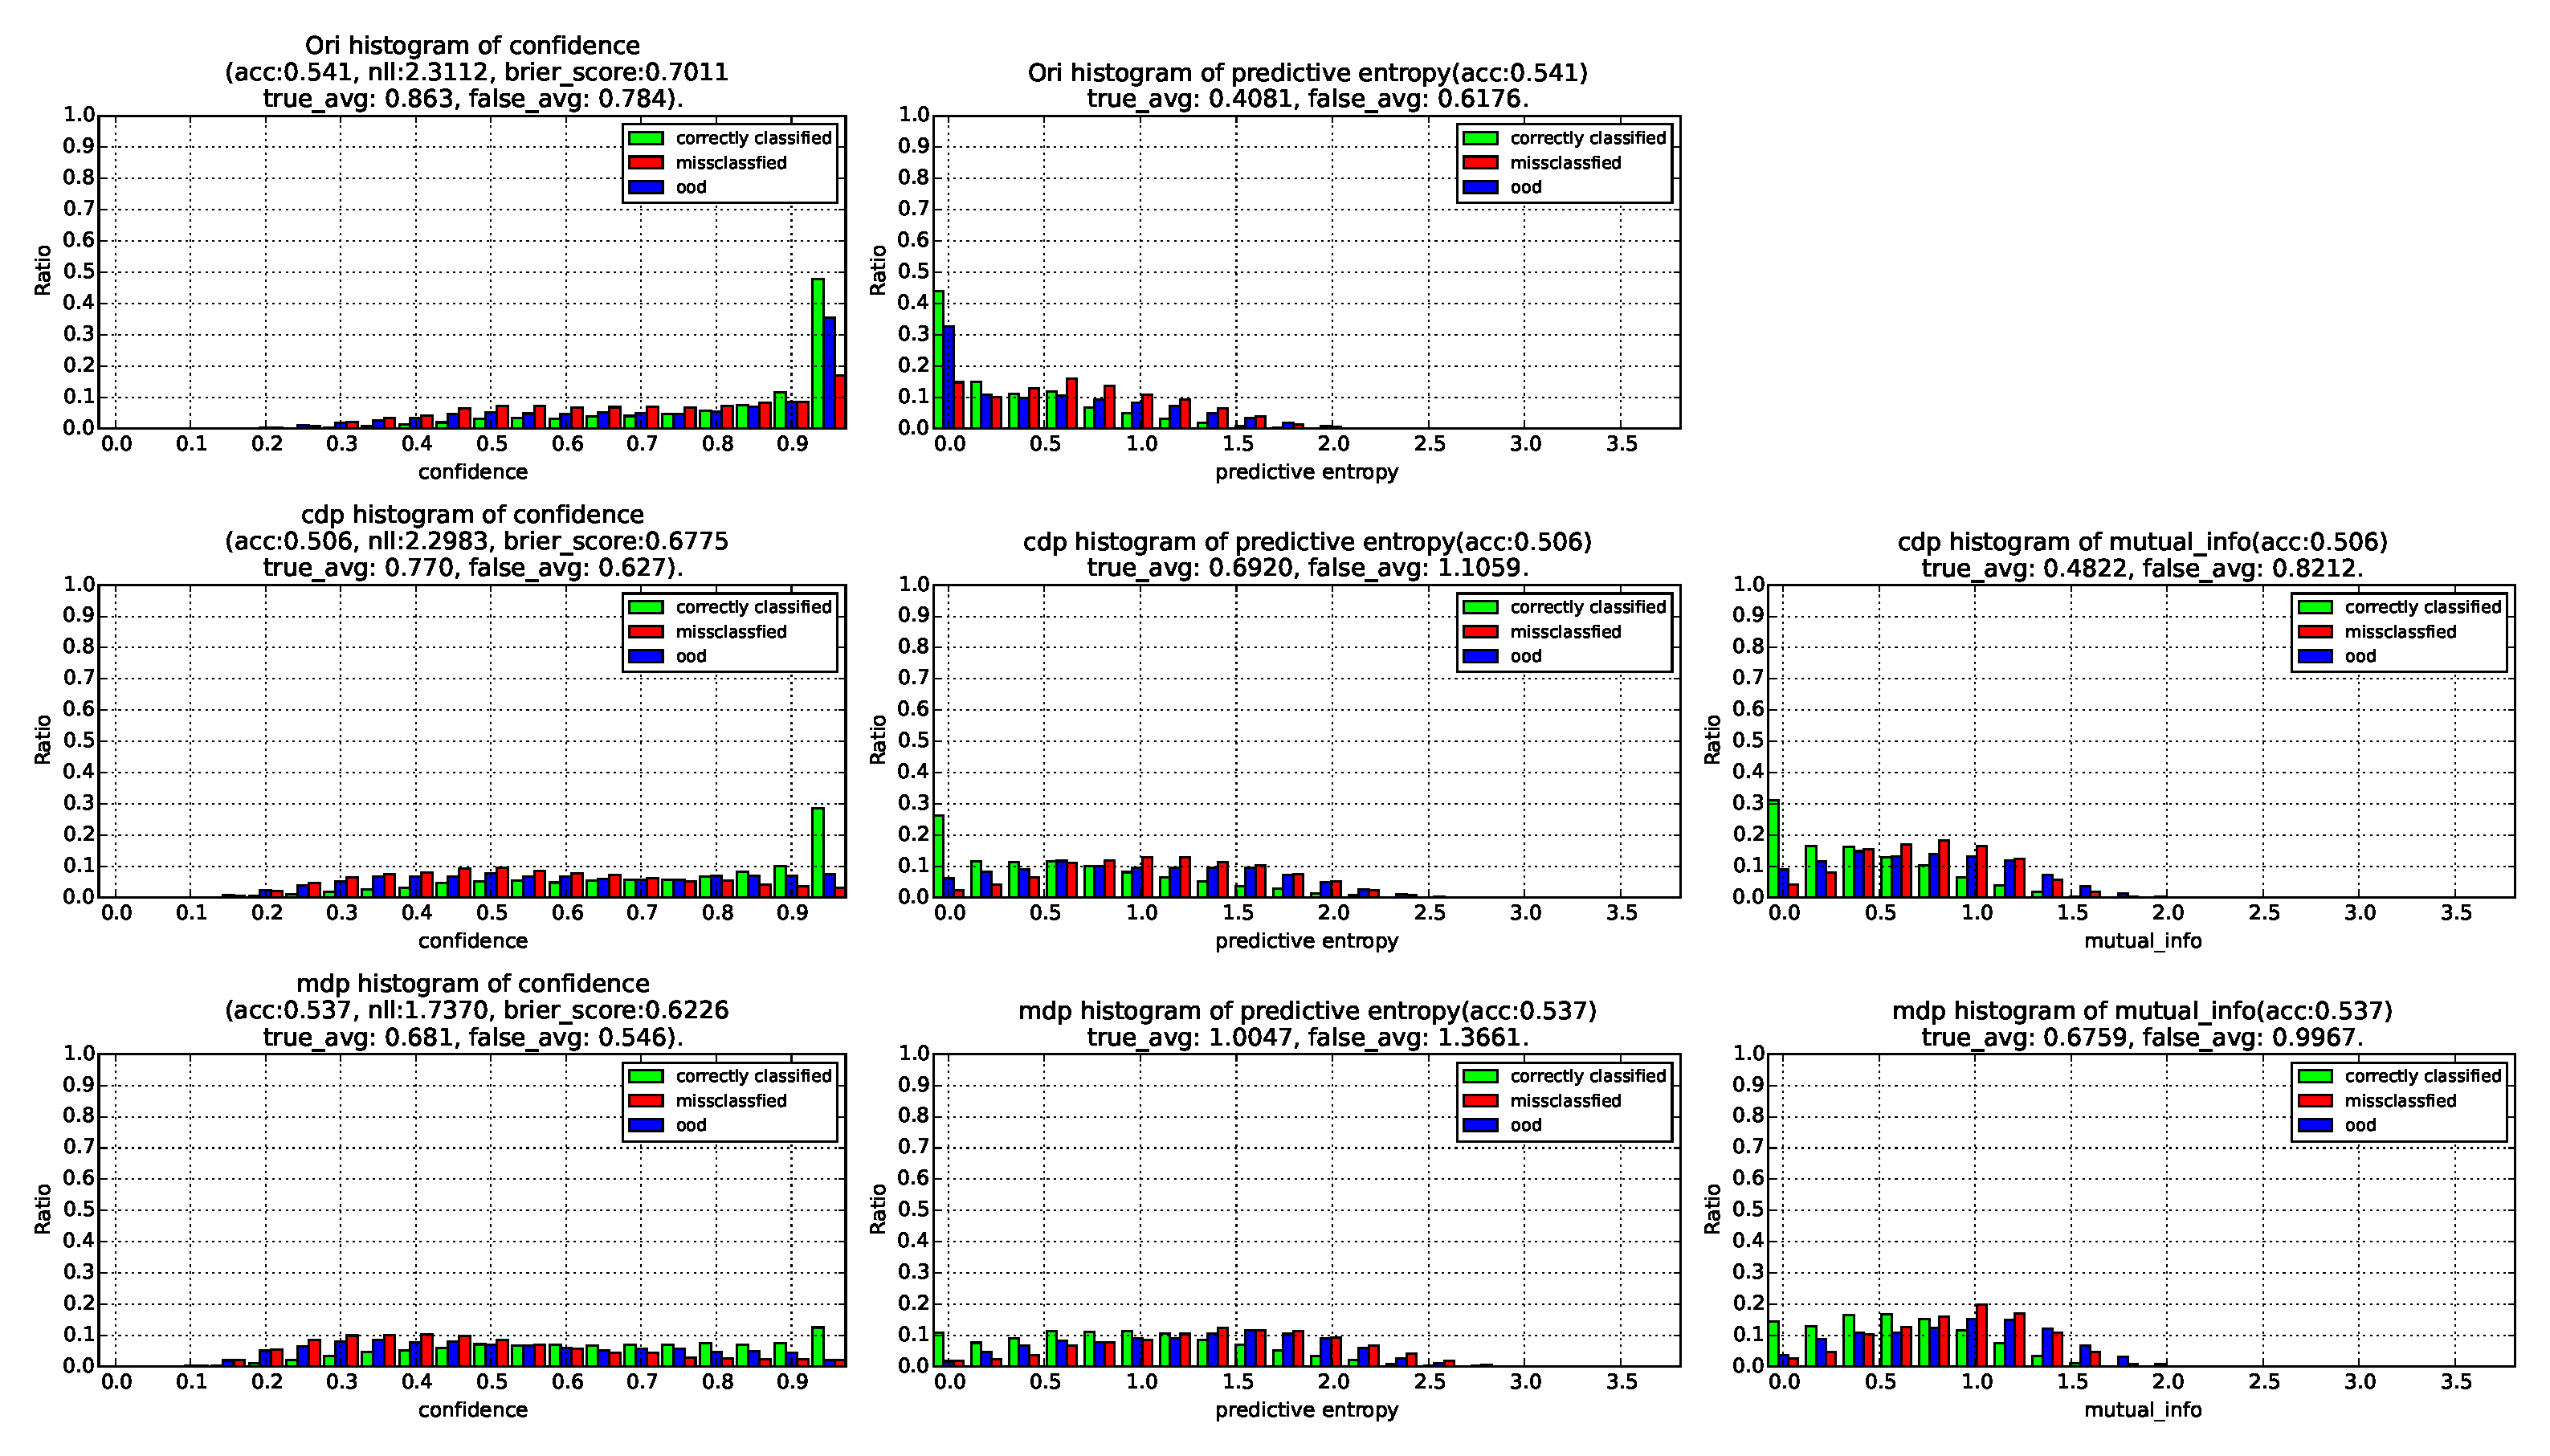
\includegraphics[height=8cm,width=16cm]{uncertainty_estimation/ablation_study/histo_froFeat_ori_cdp_mdp_ood_seed3.eps}
		\caption{Uncertainty histogram of one of three runs.}		
		\label{ab_reliability}
	\end{center}
\end{figure}


\begin{figure}[H]
	\begin{center}
		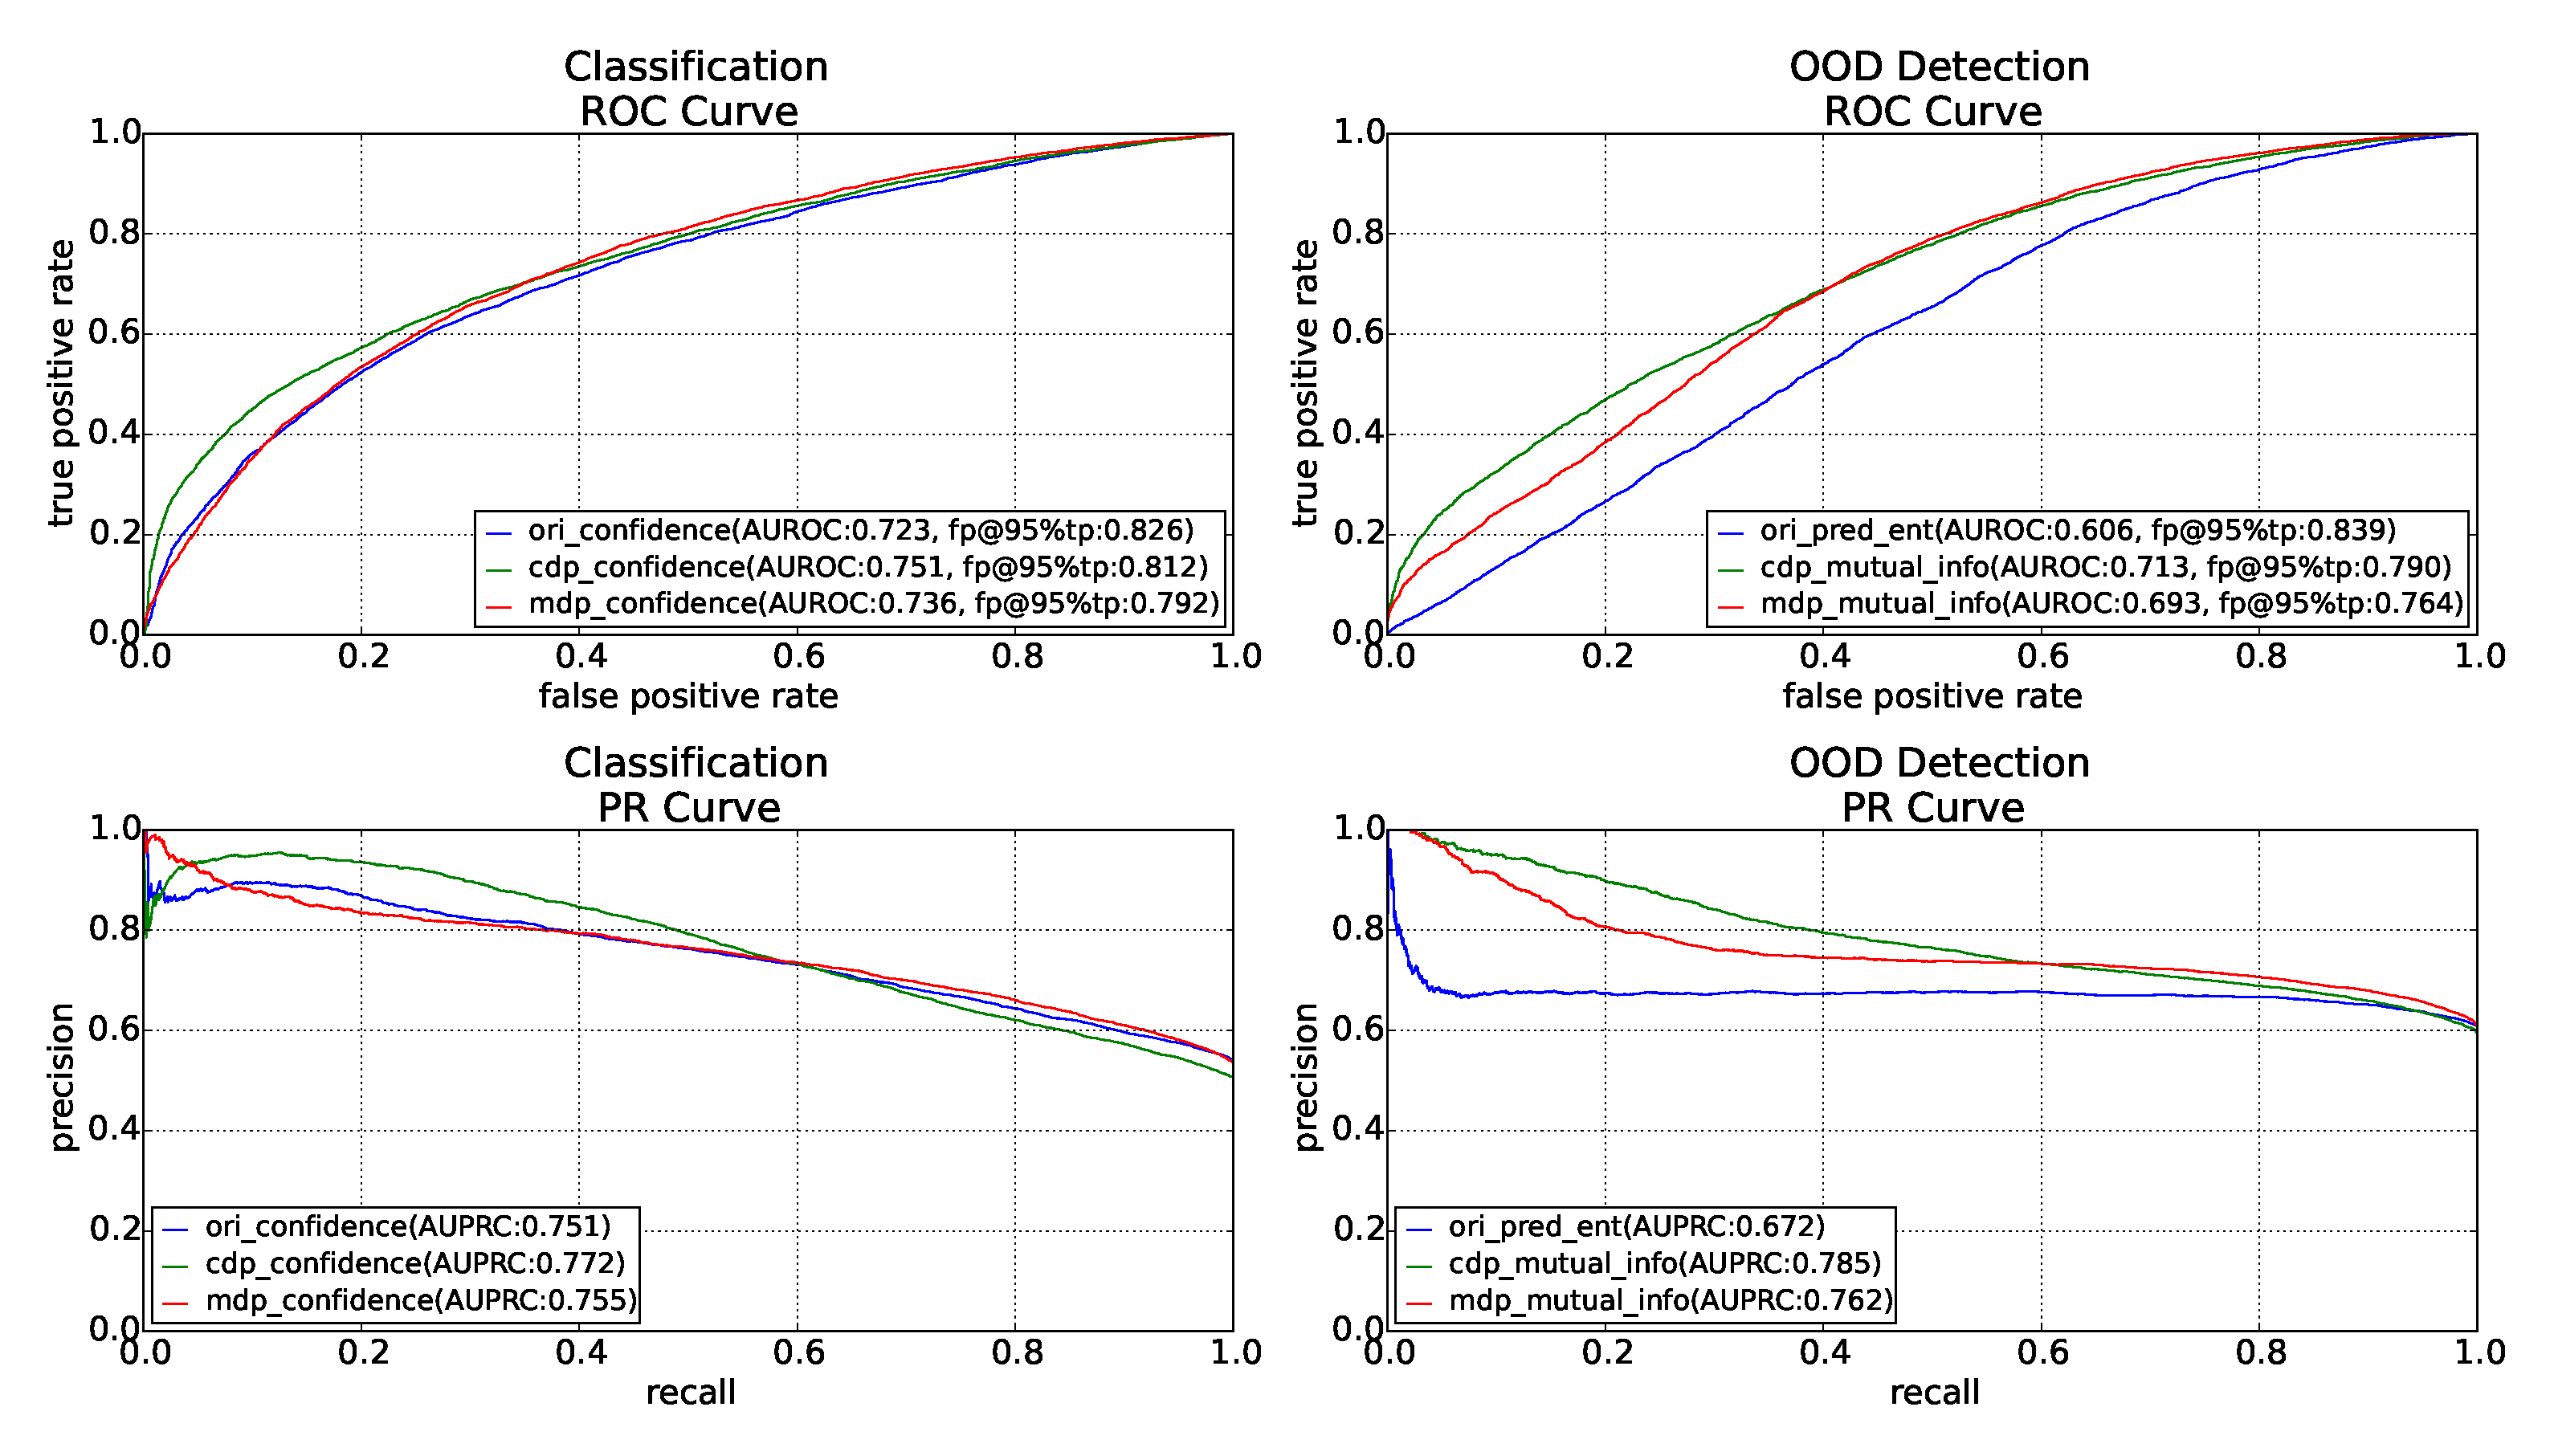
\includegraphics[height=9cm, width=16cm]{uncertainty_estimation/ablation_study/roc_pr_froFeat_ori_cdp_mdp_combined_seed3.eps}
		\caption{ROC and PR curve of one of three runs.}		
		\label{ab_roc_pr}
	\end{center}
\end{figure}
\begin{table}[H]
	\label{ab_table}
	\centering
	\caption{Quantitative results of acc, bs, nll, ece, mce, auroc, aupr.}
	\begin{tabular}{|l|l|l|l|}
		\hline
		& accuracy   $\boldsymbol \uparrow$  & brier\_score $\boldsymbol \downarrow$& \begin{tabular}[c]{@{}l@{}}negative\\ log \\ likelihood $\boldsymbol \downarrow$\end{tabular} \\ \hline
		ori           &0.532$\pm$0.015 & 0.717$\pm$0.023& 2.383$\pm$0.053                                                        \\ \hline
		cdp           & 0.521$\pm$0.011&0.655$\pm$0.017 &  2.190$\pm$0.149                                                        \\ \hline
		mdp           & 0.520$\pm$0.012 &0.641$\pm$0.014 & 1.804$\pm$0.073                                                         \\ \hline
	\end{tabular}
\end{table}

\begin{table}[H]
	\centering
	% \caption{results of ece, mce, auroc, aupr}
	\begin{tabular}{|l|l|l|l|l|}
		\hline
		& \begin{tabular}[c]{@{}l@{}}expected\\ calibration\\ error(w/o. OOD/\\ w. OOD)$\boldsymbol \downarrow$\end{tabular} & \begin{tabular}[c]{@{}l@{}}maximal\\ calibration\\ error(w/o. OOD/\\ w. OOD)$\boldsymbol \downarrow$\end{tabular} & \begin{tabular}[c]{@{}l@{}}area under\\ ROC\\ (vs. Miss-\\ classified/\\ vs. OOD)$\boldsymbol \uparrow$\end{tabular} & \begin{tabular}[c]{@{}l@{}}area under\\ PR curve\\ (vs. Miss-\\ classified/\\ vs. OOD)$\boldsymbol \uparrow$\end{tabular} \\ \hline
		ori           & \begin{tabular}[c]{@{}l@{}}0.262$\pm$0.011/ \\0.793$\pm$0.012\end{tabular}                      & \begin{tabular}[c]{@{}l@{}}0.365$\pm$0.010/ \\0.491$\pm$0.013\end{tabular}                     &
		\begin{tabular}[c]{@{}l@{}}0.716$\pm$0.005/ \\0.602$\pm$0.014\end{tabular}           & \begin{tabular}[c]{@{}l@{}}0.724$\pm$0.022/ \\0.681$\pm$0.007\end{tabular}                \\ \hline
		cdp           & \begin{tabular}[c]{@{}l@{}}0.141$\pm$0.022/ \\0.270$\pm$0.037\end{tabular}                     & \begin{tabular}[c]{@{}l@{}}0.203$\pm$0.053/ \\0.359$\pm$0.056\end{tabular}                     & \begin{tabular}[c]{@{}l@{}}0.748$\pm$0.002/ \\0.712$\pm$0.006\end{tabular}           & \begin{tabular}[c]{@{}l@{}}0.770$\pm$0.002/ \\0.782$\pm$0.004\end{tabular}                \\ \hline
		
		mdp           & \begin{tabular}[c]{@{}l@{}}0.068$\pm$0.009/ \\0.158$\pm$0.006\end{tabular}                      & \begin{tabular}[c]{@{}l@{}}0.134$\pm$0.018/ \\0.311$\pm$0.008\end{tabular}                     & \begin{tabular}[c]{@{}l@{}}0.730$\pm$0.009/ \\0.674$\pm$0.014\end{tabular}           & \begin{tabular}[c]{@{}l@{}}0.749$\pm$0.009/ \\0.748$\pm$0.010\end{tabular}                \\ \hline
	\end{tabular}
\end{table}	


\section{Automatic labeling experiments}

In experiments of automatic labeling, our goal is to perform a proof-of-concept experiment, which simulates the situation that a classifier trained on a public large scale dataset or synthetic dataset is deployed in a real world environment and tries to fine-tune itself to improve performance with automatically labeled dataset and as little manually labeled data as possible. The automatically labeled data is collected based on improved uncertainty estimation. Because ResNet50 with concrete dropout shows more stable results than other version, we use it to improve uncertainty estimation in the following experiments and call it \textbf{BNN} without other specifications. 

This way to enable the classifier to learn continuously is seldom seen in the literatures. Therefore, in order to investigate the practicability of this method, we firstly perform experiments on WRGBD and UniHB dataset with restriction on the size of collected dataset. 

Then we try to extend this way to another dataset, T-LESS dataset, to test its generalization ability in second experiment. In the second experiment, the situation is similar to the first experiment, where a classifier is firstly trained on synthetic dataset and then deployed in a real world environment which is simulated by the real objects in training set.  We employ data augmentation to address the problem of imbalance in fine-tuning classifier found in the first experiment.
 
\subsection{Experiment \RNum{1}}
The first experiment is performed on the WRGBD and UniHB dataset. As is mentioned in experiment \RNum{2} of uncertainty estimation experiments, we train classifier with entire WRGBD dataset and evaluate performance of uncertainty estimation on adaptation set from UniHB dataset, which contain the images of object of elevation $30^{\circ}$ and $60^{\circ}$, whose size is around $17.1\times10^3$. The images of $45^{\circ}$ with size $8.6\times10^3$ are used for final evaluation after fine-tuning the classifier. The dataset used for fine-tuning are collected from the adaptation set with different settings in order to investigate the issues of this way for continuous learning. 

The uncertainty measure we used is confidence because in this case we do not consider OOD data and confidence performs better in separating correct predictions and miss-classifications based on the results of previous experiments.

One major restriction we impose in this experiment is the size of dataset for fine-tuning. Because if we do not restrict the size, the performance is influenced by both the size of dataset and other factors such as imbalance or quality of dataset. In order to exclude the influence of dataset size, we fix it as 3\% of the adaptation set which is around 510. If the dataset is balanced in number of data sample of category, then there are around ten data samples in each category. The influence of other factors we want investigate are the imbalance of dataset and quality of data sample in dataset. In the following table, we use capital letter to denote different settings of dataset for fine-tuning.

Here we firstly illustrate the steps of \textbf{selecting automatically labeled data} in this experiment which is a little different to the strategy in experiment \RNum{2}. 

For C, D, E, F, G, we conduct the following steps:
\begin{itemize}
	\item[1.] Automatic labeling: select the most confident predictions and label them with their predictions.
	\item[2.] Manual labeling: select the data randomly or with least confidence required for manual labeling.
	\item[3.] Combining: combine automatically labeled and manually labeled data, then check if any category does not have data sample, if yes add one random data sample of this category.
	\item[4.] Balancing dataset: firstly check if number of data sample of any categories exceed the average number of data sample (which can be calculated beforehand), if yes, drop the data sample of this category randomly until its number reach the average number of category. After that, if augmentation is chosen, then use augmentation to increase of the number of data sample of category in which the number of data sample is less than average number of data sample.

\end{itemize}
To note that, the accuracy of automatically labeled data in C, E, F, G is around 96\%, which means not all labels of them are correct. And "\textbf{randomly}" in the context means that we randomly choose the data of each class with number computed based on the difference between current number of data samples of each class and the average number of data samples of each class. We assume that we have manually labeled all the predictions after automatic labeling and conduct a \textit{proof-of-concept} experiment with a \textbf{as balanced as possible} dataset.    


	\begin{table}[h!]
		\centering
		\label{table:fine_tuning}
		\caption{Results of fine-tuned network with different settings}
		\begin{tabular}{|l|c|}
			\hline
			Settings of dataset for fine-tuning                                                                                                                                                                                   & \multicolumn{1}{l|}{\begin{tabular}[c]{@{}l@{}}Accuracy\\ (average over 3\\ random seeds)\end{tabular}} \\ \hline
			A: 0\% (no fine-tuning)                                                                                                                                                                                                  & 66.9\%                                                                                                  \\ \hline
			\begin{tabular}[c]{@{}l@{}}B: 3\% manually labeled data randomly \\   (\textbf{balanced})\end{tabular}                                                                                                                               & 91.7\%                                                                                                  \\ \hline
			\begin{tabular}[c]{@{}l@{}}C: 3\% automatically labeled data \\ (\textbf{imbalanced})\end{tabular}                                                                                                                        & 79.0\%                                                                                                  \\ \hline
			\begin{tabular}[c]{@{}l@{}}D: 3\% manually labeled data with least confidence\\ (\textbf{imbalanced})\end{tabular}                                                                                                       & 83.3\%                                                                                                  \\ \hline
			\begin{tabular}[c]{@{}l@{}}E: 2\% automatically labeled data and \\ 1\% manually labeled data with least confidence, \\ augmentation for balance (\textbf{balanced})\end{tabular}                                     & 83.8\%                                                                                                  \\ \hline
			\begin{tabular}[c]{@{}l@{}}F: 2\% automatically labeled data and \\ 0.5\% manually labeled data with least confidence and \\ 0.5\% manually labeled data randomly,\\ augmentation for balance (\textbf{balanced})\end{tabular} & 88.3\%                                                                                                  \\ \hline
			\begin{tabular}[c]{@{}l@{}}G: 2\% automatically labeled data and \\ 1\% manually labeled data randomly,\\ augmentation for balance (\textbf{balanced})\end{tabular}                                                            & 89.6\%                                                                                                  \\ \hline
		\end{tabular}
	\end{table}
From the description of settings we know that predictions with most confidence and least confidence are imbalanced in number of data sample of each category. Based on the results in the table \ref{table:fine_tuning}, we can obtain the following observations:
\begin{itemize}
	\item diverse and balanced dataset can achieved best performance.
	\item the difference of performance between C and D may attribute to quality of dataset which include correct labeling and information of data sample.
	\item by comparing performance of E, F and G, we know that diverse data sample before augmentation is important to achieve better performance. When considering information of data sample, manually labeling of lest confident data sample sounds better. However, we also know that before augmentation dataset in E is more imbalanced than that in F, and F is more imbalanced than G because of the higher proportion of predictions with least confidence. Therefore it shows that data balance is more important than information of data sample in this case.
\end{itemize}
By comparing the results of other settings with that of A and B, we can see that the manual labeling effort can be reduced based on automatic labeling.  The performance of fine-tuned domain specific classifier can nearly reach the the performance of classifier fine-tuned with all manually labeled data. 

In the end, we can draw a conclusion that diversity of data and balance of number of data sample of each category play an significant role. Based on the last aforementioned observation, balance of number of data sample of each category is more important in than information of data sample.

\subsection{Experiment \RNum{2}}
In this experiment, we firstly train networks on synthetic and augmented dataset which is introduced previously. Then we select automatically labeled data by testing the trained model on real single objects (original training set of T-LESS) which we call \textbf{adaptation dataset}. The difference between the strategy of selecting data in experiment \RNum{1} is that we split off a small balanced validation set from the whole real single object dataset with ratio 1:9. Then we choose the threshold of uncertainty up to which the accuracy can reach 95\% based on predictions on validation set. This threshold is employed in the rest of whole adaptation dataset for selecting automatically labeled data. In this experiment we use predictive entropy as uncertainty measure, because it shows better performance in term of separability metrics on validation set.

The improved uncertainty estimation from BNN plays an important role here, because it not only provides a reliable uncertainty estimation, but also increases the separability between correct predictions and false predictions, which is more useful in this task. 

We show the comparisons in term of different evaluation metrics between uncertainty estimation from BNN and original ResNet50 in the following figures. As we can see in the uncertainty histogram (cf.\ref{autoLa_exp2_hist}), the mode of distribution of uncertainty estimation between correct prediction and miss-classification is further from each other when testing with BNN than with original ResNet50. In figure \ref{autoLa_exp2_cali}, BNN express better performance on both calibration and separability metrics. 

With the same procedure of selecting automatically labeled data, we can only obtain around $1.05\times10^3$ data samples with only 93\% accuracy using original ResNet50, but around $1.6\times10^3$ data samples with 96\% accuracy using BNN. Therefore we do not consider fine-tuning with original ResNet50 here and focus on fine-tuning BNN.

\begin{figure}[H]
	\begin{center}
		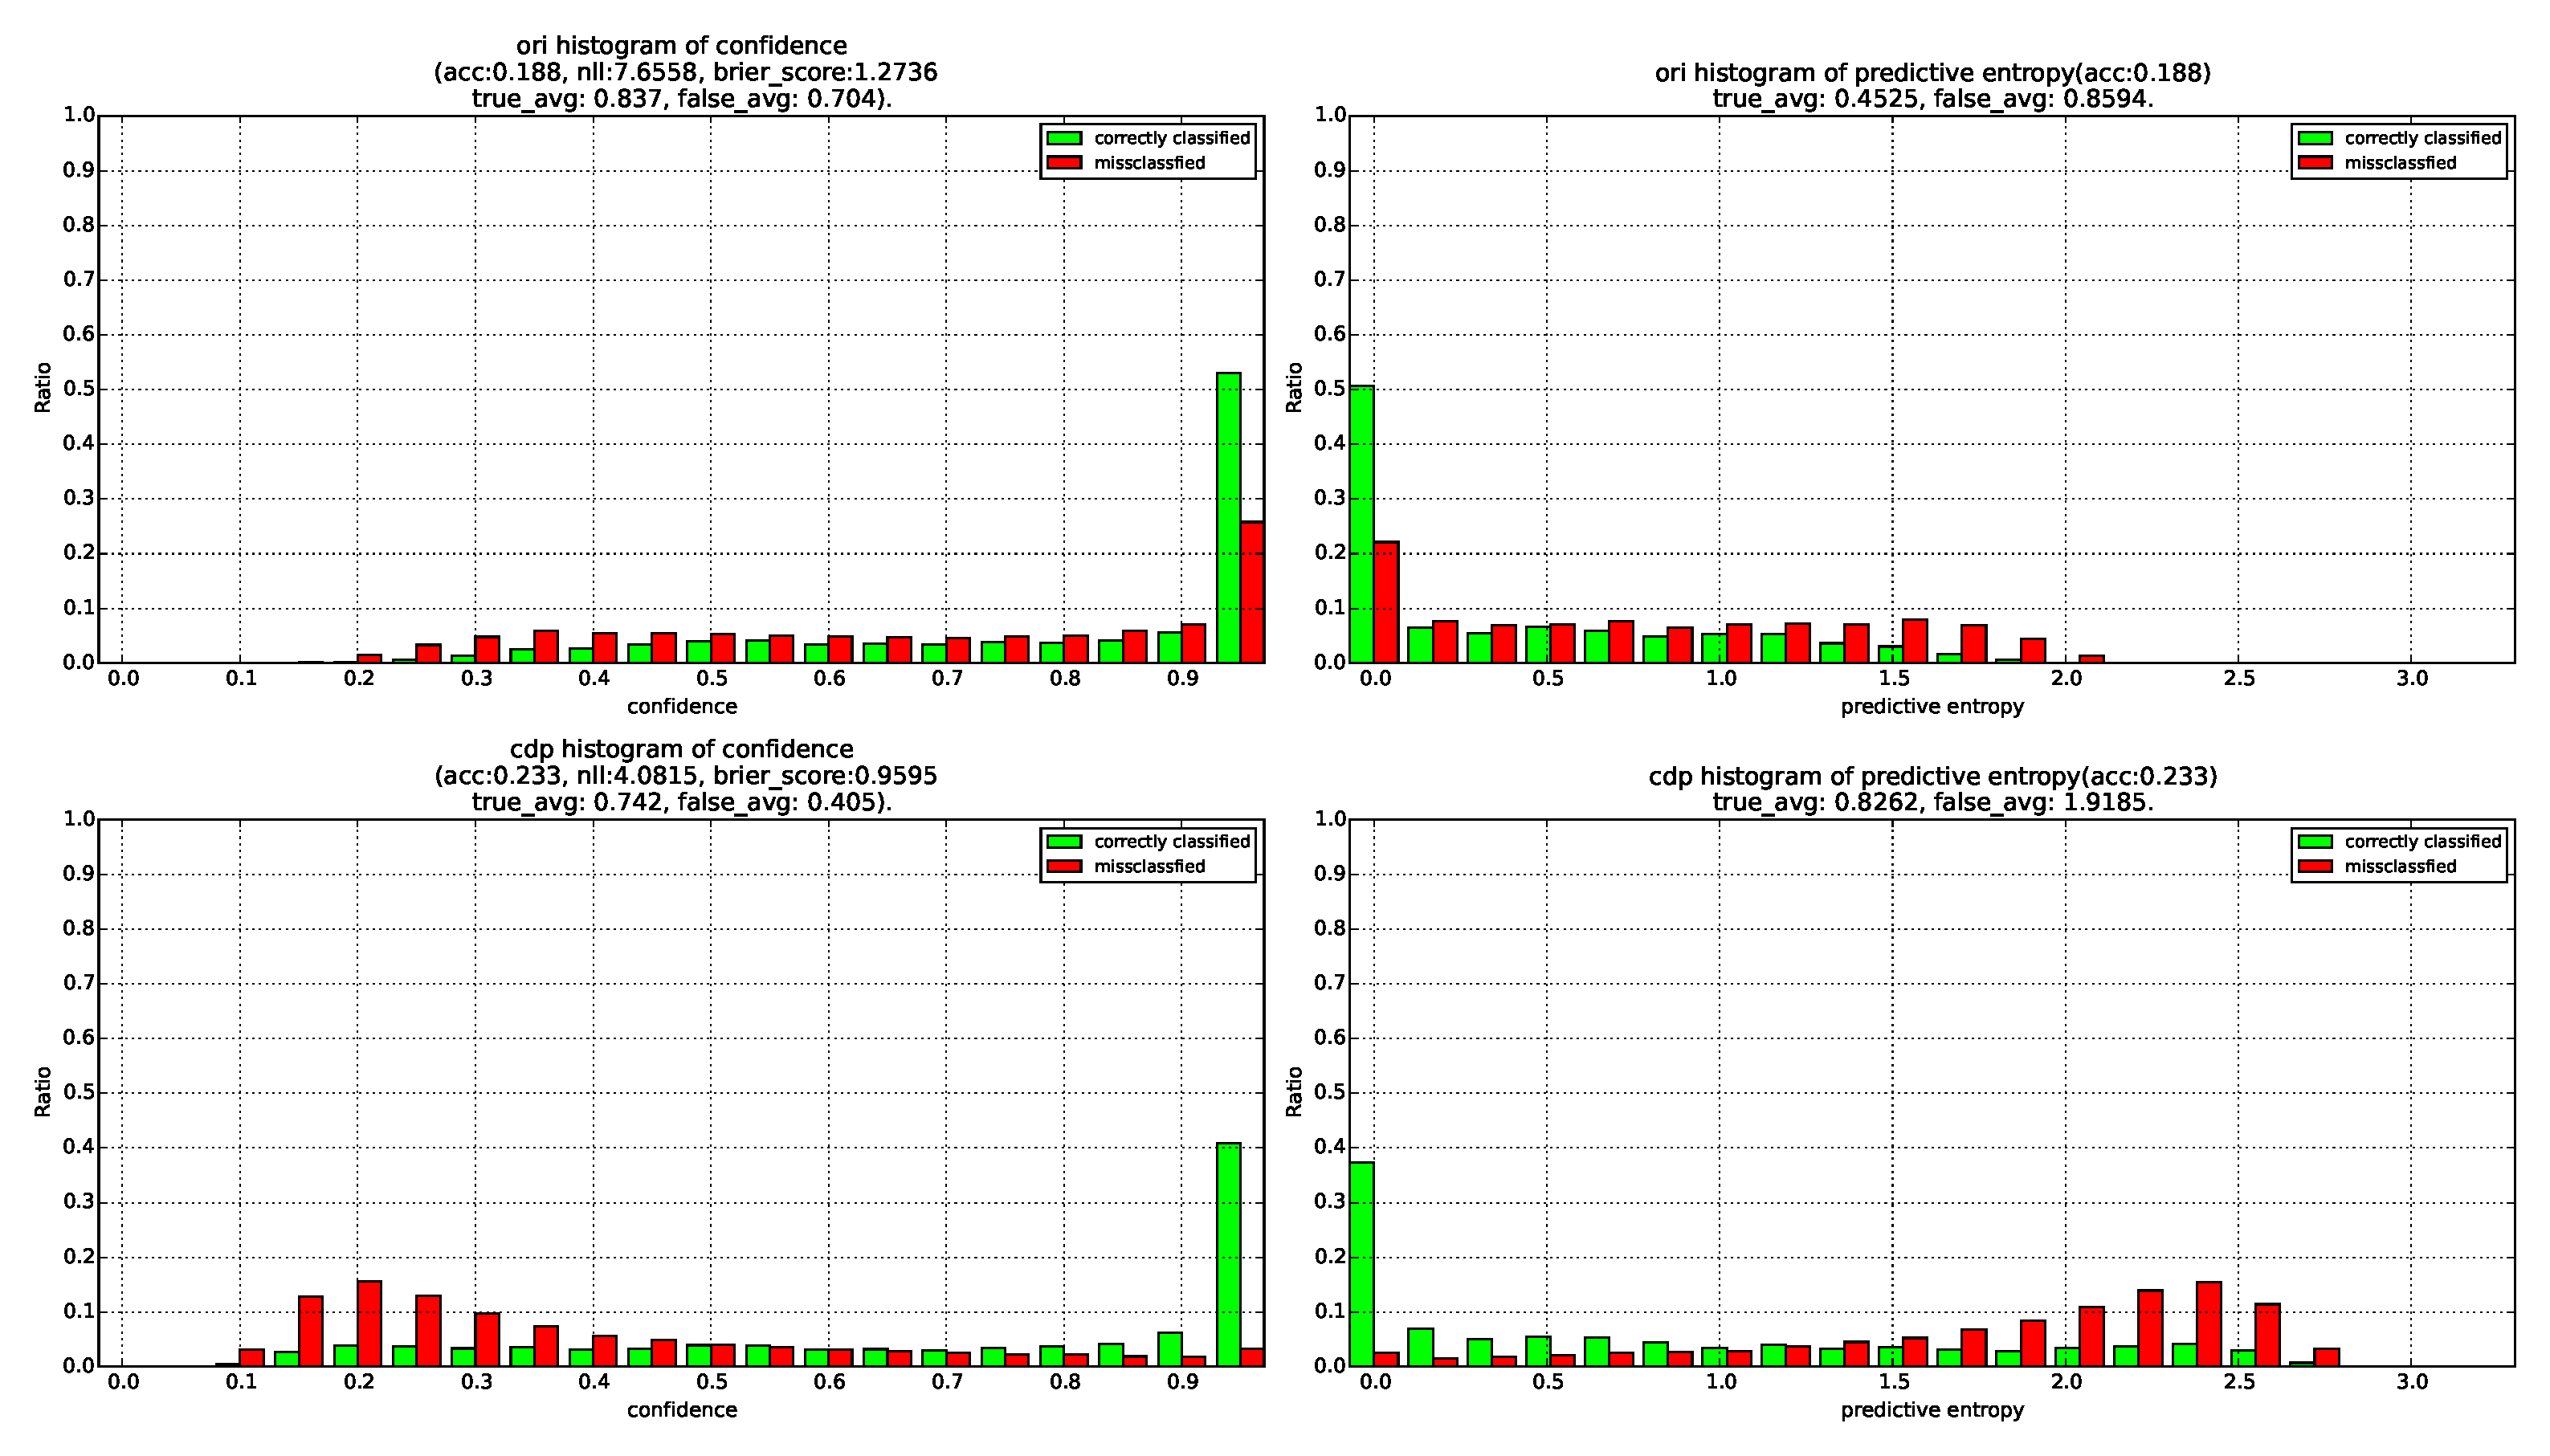
\includegraphics[height=6.7cm,width=12cm]{autoLa/exp2/uncer_hist.eps}
		\caption{Uncertainty histograms of original ResNet50 (top)and BNN (down).}		
		\label{autoLa_exp2_hist}
	\end{center}
\end{figure}
However, as we found in experiment \RNum{1}, the problem of imbalance in number of data samples of each class still appears on this dataset. The confusion matrix in figure \ref{autoLa_exp2_cfm} shows this problem obviously, in which most of confident predictions cluster in few classes. To mitigate this problem, we adopt two simple ways which have been tested in experiment \RNum{1}:
\begin{itemize}
\item manually label data uniformly with size 3\% of the adaptation set.
\item employ augmentations, occlusions and different background images to the objects to make the selected dataset balanced.  
\end{itemize} 

\begin{figure}[H]
	\begin{center}
		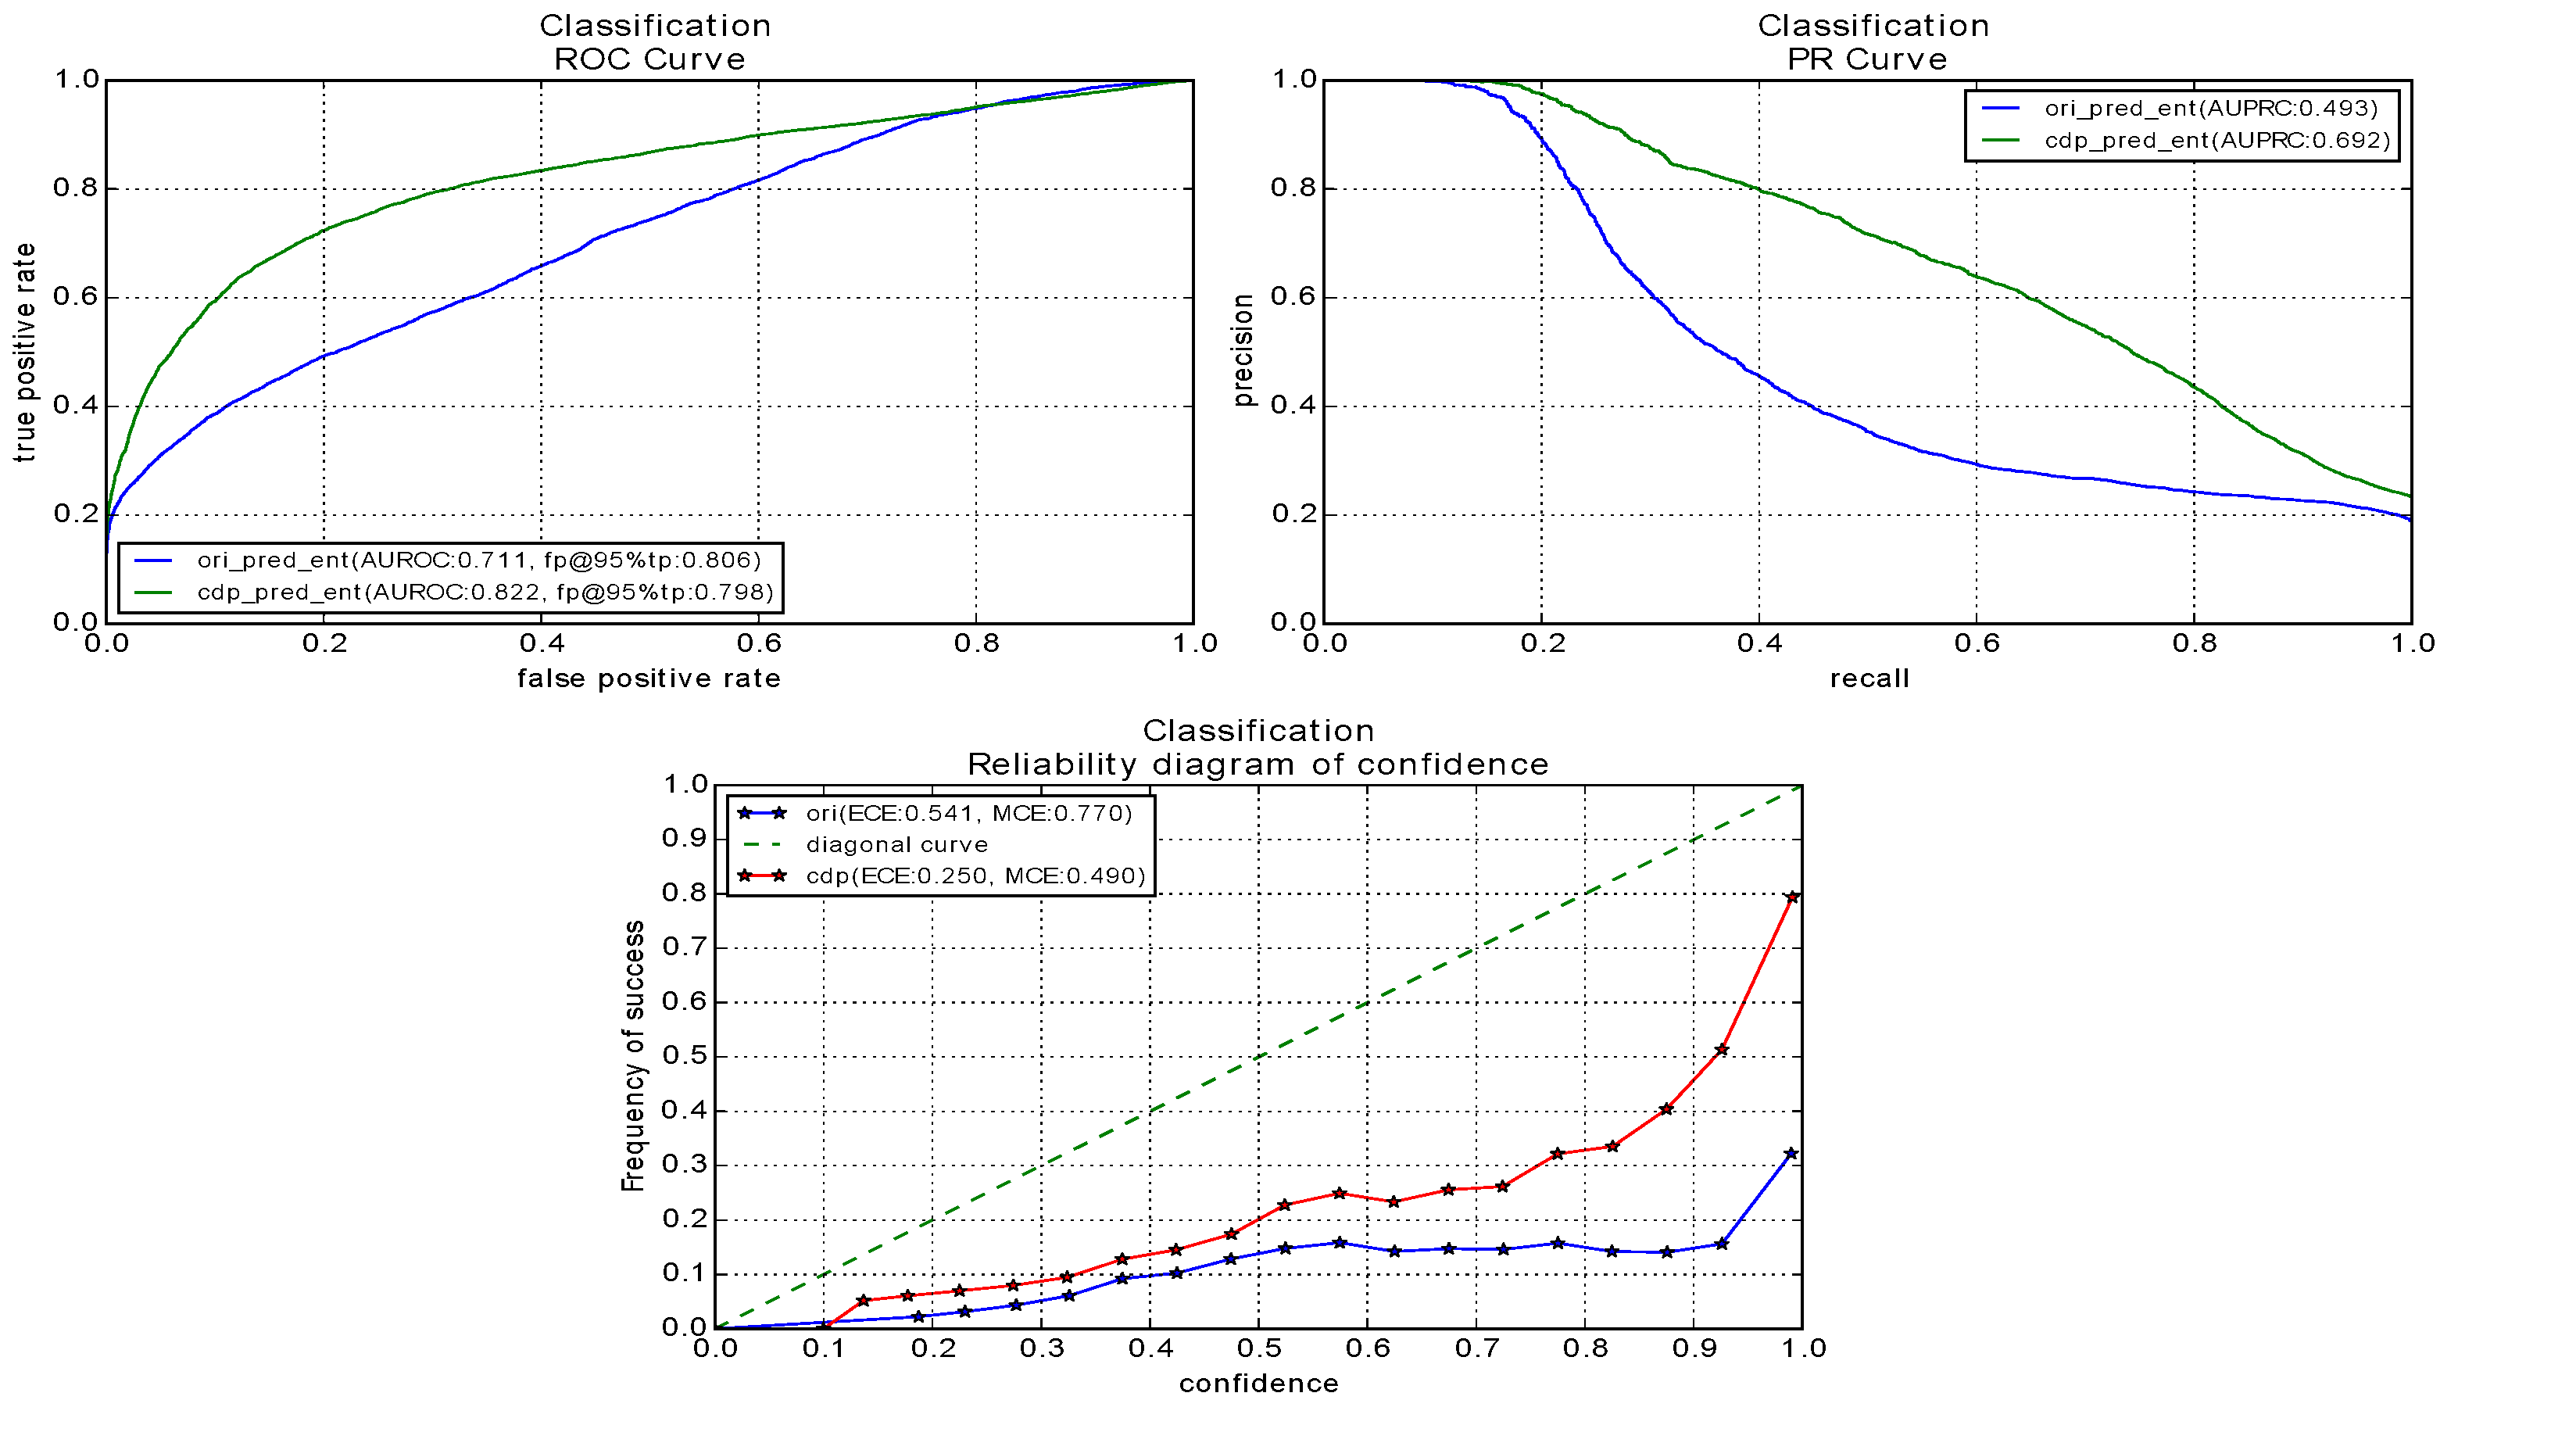
\includegraphics[height=8cm,width=14cm]{autoLa/exp2/roc_pr_cali_.eps}
		\caption{Calibration curves, ROC curves, PR curves.}		
		\label{autoLa_exp2_cali}
	\end{center}
\end{figure}


\begin{figure}[H]
	\centering
	\begin{center}
		\includegraphics[height=7cm,width=13cm]{autoLa/exp2/cmf.eps}
		\caption{Confusion matrix of automatically labeled dataset.}		
		\label{autoLa_exp2_cfm}
	\end{center}
\end{figure}


\section{Context-based improvement experiments}
In this section, we perform experiments to investigate the effect of improved uncertainty estimation when incorporating them with a probabilistic graphical model in down-stream task. In detail, we employ CRF introduced in chapter 3 to capture the dependencies between objects by exploiting contextual information in the scene. The intuition behind this idea is that if the predictive distribution (used as one uncertainty measure) is more reliable and can represent the inherent randomness better. Then this bit of information can be better utilized by CRF in the down-stream task. Similar to previous experiment, we use ResNet50 with concrete dropout to improve uncertainty estimation in the following experiments and call it \textbf{BNN} without other specifications.

As is mentioned in chapter 3, we modify CRF library \cite{Ruiz-Sarmiento-REACTS-2015} for the experiments, in which loopy belief propagation is employed both during training and testing. We have done mainly two experiments in this part. Firstly we perform a simpler experiment on subset of T-LESS dataset to show that CRF can capture the dependencies and then improve the performance. The performance can be boosted with improved uncertainty estimation from Bayesian neural network. Secondly, we test the same idea on the entire T-LESS dataset based on the output of classifier fine-tuned in the automatic labeling experiment. 


\subsection{Experiment \RNum{1}}
In this experiment, we train original ResNet50 and BNN on the real single objects with black background which is the original training set of T-LESS dataset. Then we use a subset of test scenes to train and test CRF. In detail, we use scene 1, 2, 3, 4 to train CRF, and use scene 5, 6, 7, 8 to test CRF. The background of these scenes are black, thus we do not apply augmentations to the dataset for training the CRF. Regarding the hyper-parameters in training CRF, we set size of mini-batch as 16, learning rate as $1e^-4$ and maximum number of iteration as $15\times10^3$. As is mentioned in chapter 3, we perform optimization with stochastic gradient descent(SGD) with momentum and loopy belief propagation(LBP) for inference. The maximum number of iteration for computing messages in LBP is 100, and the convergence threshold is $1e^{-4}$. In experiments, the algorithm always reach the maximum number of iteration during optimization.

In the table \ref{table:crf_exp1_acc}, we show the results of CRF trained with two different unary features from two different versions of ResNet50 and tested on scene 5, 6, 7, 8. As we can see, the network trained and tested with unary feature from BNN can yield more improvement(13.17\%) compared with that from deterministic network (12.42\%).  

 \begin{table}[H]
 	\centering
 	\caption{Results of CRF trained with unary feature from different versions of ResNet50}
 	\label{table:crf_exp1_acc}
 	\begin{tabular}{|c|c|c|}
 		\hline
 		\multicolumn{1}{|l|}{}                                            & \begin{tabular}[c]{@{}c@{}}accuracy with\\ unary\\ potential\end{tabular} & \begin{tabular}[c]{@{}c@{}}accuracy with\\ unary and pariwise\\ potentials\end{tabular} \\ \hline
 		\begin{tabular}[c]{@{}c@{}}unary feature \\ from ori\end{tabular} & 48.79\%                                                                   & 61.21\%                                                                                 \\ \hline
 		\begin{tabular}[c]{@{}c@{}}unary feature \\ from BNN\end{tabular} & 51.94\%                                                                   & 65.11\%                                                                                 \\ \hline
 	\end{tabular}
 \end{table}
Additionally, because the weights in our CRF model act as coefficients for two kinds of features, we can check the magnitude of these two weights which can indicate the contribution to overall performance. In the table \ref{table:crf_exp1_weights}, we can see that in CRF trained with unary feature from BNN, the weight of unary feature $\theta_u$ is larger than the one of edge feature $\theta_p$. The situation is inverse in CRF trained with unary feature from deterministic ResNet50. This means that the unary feature contributes more than the pairwise one if we use the predictive distribution from BNN. It also shows that the predictive distribution from BNN contains more information than its counterpart from deterministic one. More importantly, this information can be utilized to improve the performance which is shown in the table \ref{table:crf_exp1_acc}.
\begin{table}[H]
	\centering
	\caption{Learned weights of CRF trained with unary feature from different versions of ResNet50}
	\label{table:crf_exp1_weights}
	\begin{tabular}{|c|c|c|}
		\hline
		\multicolumn{1}{|l|}{}                                            & \begin{tabular}[c]{@{}c@{}}node weight\\ $\theta_u$ \end{tabular} & \begin{tabular}[c]{@{}c@{}}edge weight\\ $\theta_p$ \end{tabular} \\ \hline
		\begin{tabular}[c]{@{}c@{}}unary feature \\ from ori\end{tabular} & 3.744                                                   & 4.213                                                   \\ \hline
		\begin{tabular}[c]{@{}c@{}}unary feature \\ from BNN\end{tabular} & 4.635                                                   & 3.882                                                   \\ \hline
	\end{tabular}
\end{table}

\subsection{Experiment \RNum{2}}
In this experiment, we want to test the generalization ability of CRF on the whole T-LESS dataset.
